%==============================================================
%Encap�alament
%==============================================================
\documentclass[a4paper,oneside,12pt]{article}
\usepackage[left=2.5cm,right=2cm,top=2cm,bottom=2cm]{geometry}
\usepackage[catalan]{babel}
\usepackage[T1]{fontenc}
\usepackage[latin1]{inputenc}
\usepackage{graphicx} % Required for including pictures
\usepackage{subfigure} % subfiguras
\usepackage{float} % Allows putting an [H] in \begin{figure} to specify the exact location of the figure
\usepackage{wrapfig} % Allows in-line images
\linespread{1.2}
\graphicspath{{Pictures/}}

\usepackage{subscript} %super�ndexs i sub�ndexs
\setcounter{secnumdepth}{5} %Numerar fins a subpar�grafs
\usepackage{pdfpages} %posar arxius pdf (com articles...)

\usepackage{amssymb, amsmath, amsbsy} % librerias ams
\usepackage{stackrel} %Escriure a sobre o sota de qualsevol fletxa
\usepackage{color}
\usepackage{multicol}
\usepackage{array}
\usepackage[full]{textcomp}
\usepackage{multirow}

% Enumeracions
\usepackage[shortlabels]{enumitem}
\usepackage{pstricks}

\usepackage{tikz}
\newcommand*{\itembolasazules}[1]{% bolas 3D 
	\footnotesize\protect\tikz[baseline=-3pt]% 
	\protect\node[scale=.7, circle, shade, ball
	color=blue]{\color{white}\Large\bf#1};}

\newcommand*{\itembolasverdes}[1]{% bolas 3D 
	\footnotesize\protect\tikz[baseline=-3pt]% 
	\protect\node[scale=.7, circle, shade, ball
	color=green]{\color{white}\Large\bf#1};}

\newcommand*{\itembolasrojas}[1]{% bolas 3D 
	\footnotesize\protect\tikz[baseline=-3pt]% 
	\protect\node[scale=.7, circle, shade, ball
	color=red]{\color{white}\Large\bf#1};}

% Lletres gregues
\DeclareRobustCommand{\greektext}{%
  \fontencoding{LGR}\selectfont\def\encodingdefault{LGR}}
\DeclareRobustCommand{\textgreek}[1]{\leavevmode{\greektext #1}}
\DeclareFontEncoding{LGR}{}{}
\DeclareTextSymbol{\~}{LGR}{126}

%Bibliografia
\usepackage[square]{natbib}

% Instruccions especials
\newcommand{\seny}{senyalitzaci�}
\newcommand{\aas}{amino�cids}
\newcommand{\TF}{factor de transcripci�}
\newcommand{\TFs}{factors de transcripci�}
\newcommand{\tgfb}{TGF\textgreek{b}}
\newcommand{\pparg}{PPAR\textgreek{g}}
\newcommand{\betaadren}{\textgreek{b}-adren�rgic}
\newcommand{\Rbeta}{R\textsubscript{\textgreek{b}}}
\newcommand{\iso}{isoproterenol}
\newcommand{\aden}{adenilat ciclasa}
\newcommand{\ca}{Ca\textsuperscript{2+}}
\newcommand{\betacat}{\textgreek{b}-catenina}
\newcommand{\fletsup}{$\uparrow$}
\newcommand{\fletinf}{$\downarrow$}
\newcommand{\gng}{gluconeog�nesi}
\newcommand{\tnfa}{TNF-\textgreek{a}}
\newcommand{\ikb}{I\textgreek{k}B\textgreek{a}}
\newcommand{\nfkb}{NF-\textgreek{k}B}
\newcommand{\pgc}{PGC-1\textgreek{a}}
\newcommand{\na}{Na\textsuperscript{+}}
\newcommand{\pot}{K\textsuperscript{+}}
\newcommand{\ags}{�cids grassos}
\newcommand{\ck}{cicle de Krebs}
\newcommand{\ag}{�cid gras}
\newcommand{\ppara}{PPAR\textgreek{a}}
\newcommand{\ppard}{PPAR\textgreek{d}}
\newcommand{\ifng}{IFN-\textgreek{g}}

% F�rmules qu�miques
\usepackage{chemformula}
%\usepackage[version=4,arrows=pgf]{mhchem}
\usepackage{texshade}
\usepackage{textopo}

%\newcommand{\powd}[1]{$10^{#1}$}
%\newenvironment{?}{?}{?}

\setcounter{tocdepth}{2} % numerar fins subseccions a TOC

% Encap�alament i peu de p�gina
\usepackage{fancyhdr}
\pagestyle{fancy}
%\renewcommand{\sectionmark}[1]{\markright{\textsc{\thesection. #1}}}
\lhead{}
\rhead{}
\lfoot{\sc Bioqu�mica Anal�tica i Cl�nica}
%\rfoot{\thepage}
\cfoot{}

\fancyfoot[R]{\thepage}

\renewcommand{\headrulewidth}{0.4pt}
\renewcommand{\footrulewidth}{0.4pt}

\raggedbottom
\providecommand{\tabularnewline}{\\}


% Format seccions
%\usepackage{sectsty}
%\sectionfont{\centering\nohang\LARGE\bfseries}
%\partfont{\centering\huge\red}
\usepackage{titlesec}

\titleformat{\section}[block]{\centering}{\bfseries\LARGE\thesection  . }{0em}{\LARGE\bfseries}{}

\titleformat{\subsection}[hang]{\flushleft}{\bfseries\Large\thesubsection }{0.2cm}{\Large\bfseries}

\titleformat{\subsubsection}[hang]{\flushleft}{\bfseries\large\thesubsubsection }{0.2cm}{\large\bfseries}

% Format parts
%\titleformat{\part}[hang]{\centering\vspace{-1.75cm}}{\bfseries\huge\thepart . }{0em}{\huge \bfseries}{}
\newcommand{\titline}{\titlerule[2pt]}
\titleformat{\part}[hang]
  {\vspace{-2cm}\sc\bfseries\huge\red}{\centering\huge\sc\bfseries
  	}
  {0ex}
  {\titline \\
   \vspace{1pt}%
   \centering\huge\sc\bfseries\red\thepart . }
   [%
 \titline]

\usepackage[hyperindex,linktocpage]{hyperref}

% Format �ndex
\usepackage{kpfonts}
\usepackage{titletoc}
\contentsmargin{0cm}
\titlecontents{part}[0pc]
{\addvspace{30pt}%
	\\\color{red}\large\sc\bfseries}%
{}
{}
{\;\titlerule\;\large\bfseries \thecontentspage}%
\titlecontents{section}[2.4pc]
{\addvspace{1pt}}
{\bfseries\contentslabel[\thecontentslabel]{2.4pc}}
{}
{\hfill\small\bfseries\thecontentspage}
[]
\titlecontents*{subsection}[4pc]
{\addvspace{-1pt}\small}
{}
{}
{\ --- \small\thecontentspage}
[ \textbullet\ ][]
%%--


% ====================ENTORNS ====================
\usepackage{tikz,tkz-tab}
\usepackage{tcolorbox, empheq}%

% Entorn per dades
\definecolor{colordadesfons}{RGB}{255,255,255}
\definecolor{colordadesmarc}{RGB}{108, 217, 0}

%\definecolor{colorrecfons}{RGB}{203,216,227}
\definecolor{colorrecfons}{RGB}{255,255,255}
\definecolor{colorrecmarc}{RGB}{128,177,221}

\tcbuselibrary{theorems}
\newtcbtheorem[number within=section]{dades}{An�lisi de dades} {colback=colordadesfons,colframe=colordadesmarc,fonttitle=\bfseries,separator sign={\ $\blacktriangleright$}}{theo}

\newtcbtheorem[number within=section]{rec}{Recordatori} {before=\begin{center},after=\end{center},colback=colorrecfons,colframe=colorrecmarc,fonttitle=\bfseries,separator sign={\ $\blacktriangleright$}}{theo}

\newtcbtheorem[number within=section]{metodes}{M�todes} {colback=red!5!white,colframe=red!75!black,fonttitle=\bfseries,separator sign={\ $\blacktriangleright$}}{theo}

% Equacions
\tcbuselibrary{skins,breakable}
\newcounter{example}
\colorlet{colexam}{red!75!black}

\newtcolorbox[]{myexample}[2][]{%
	empty,title={#1 \thetcbcounter},attach boxed title to top left,
	boxed title style={empty,size=minimal,toprule=2pt,top=4pt,
		overlay={\draw[colexam,line width=2pt]
			([yshift=-1pt]frame.north west)--([yshift=-1pt]frame.north east);}},
	coltitle=colexam,fonttitle=\Large\bfseries,
	before=\par\medskip\noindent,parbox=false,boxsep=0pt,left=0pt,right=3mm,top=4pt,
	breakable,pad at break*=0mm,vfill before first,
	overlay unbroken={\draw[colexam,line width=1pt]
		([yshift=-1pt]title.north east)--([xshift=-0.5pt,yshift=-1pt]title.north-|frame.east)
		--([xshift=-0.5pt]frame.south east)--(frame.south west); },
	overlay first={\draw[colexam,line width=1pt]
		([yshift=-1pt]title.north east)--([xshift=-0.5pt,yshift=-1pt]title.north-|frame.east)
		--([xshift=-0.5pt]frame.south east); },
	overlay middle={\draw[colexam,line width=1pt] ([xshift=-0.5pt]frame.north east)
		--([xshift=-0.5pt]frame.south east); },
	overlay last={\draw[colexam,line width=1pt] ([xshift=-0.5pt]frame.north east)
		--([xshift=-0.5pt]frame.south east)--(frame.south west);},% 
}

\begin{document}

%----------------------------------------------------------
%Portada
%----------------------------------------------------------
\begin{titlepage}

\newcommand{\HRule}{\rule{\linewidth}{0.5mm}} % Defines a new command
                                % for the horizontal lines, change
                                % thickness here 

\center % Center everything on the page
\HRule \\[0.4cm]
{\Huge\bfseries\textsc{Bioqu�mica Anal�tica i Cl�nica}} \\[0.4cm] % Title of your document
\HRule \\[04cm]
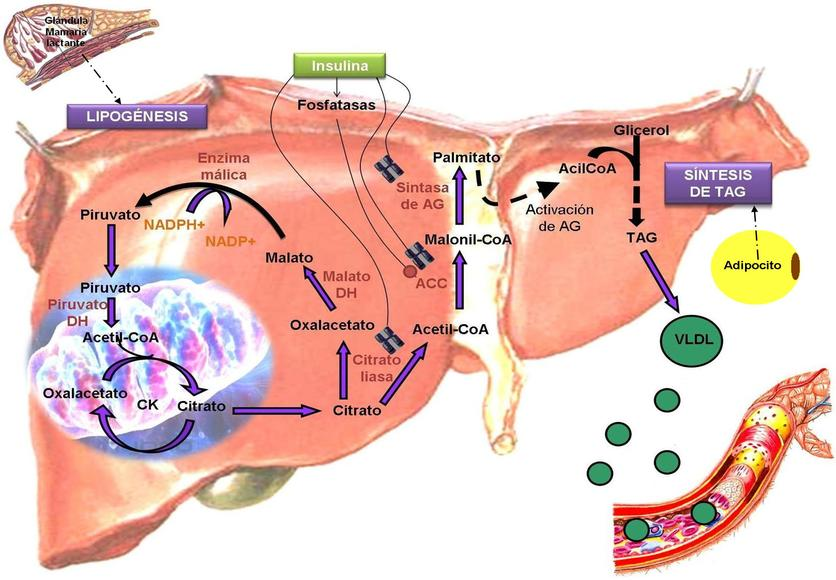
\includegraphics[width=1\textwidth]{Logo} %Include a department/university logo

\vspace{1cm}
\textsc{\Large Ci�ncies Biom�diques UB - Primavera 2017}\\[0.5cm] % Minor heading such as course title
\vspace{0.5cm}
\textsc{\large Albert Torell� P�rez}
\vfill % Fill the rest of the page with whitespace
\end{titlepage}

%===================================
\renewcommand{\figurename}{\textsc{{Figura}}}
\renewcommand{\tablename}{\textsc{{Taula}}}
\renewcommand{\thefootnote}{\alph{footnote}}

%------------------------------------------------------------------------------
%Cos dels apunts 
%------------------------------------------------------------------------------
\pagenumbering{Roman} % para comenzar la numeraci�n de paginas en
                      % n�meros romanos 

%----------------------------
% Taula de continguts
%----------------------------
\tableofcontents

\pagenumbering{arabic}
%------------------------------------------------------------------------------
% Tema 1. Variabilitat Cl�nica
%------------------------------------------------------------------------------
\newpage
%------------------------------------------------------------------------------
% Tema 1. Embrionic Stem Cells
%------------------------------------------------------------------------------
\section{\textit{Embrionic Stem Cells}}
D'una cèl·lula embrionària és interessant obtenir-ne clons. Dels diferents clons que s'obtenen s'ha de comprovar la pluripotencialitat.

Una \textbf{stem cell} és una cèl·lula que presenta 2 propietats (poden ser endògenes o induïdes):
\begin{enumerate}
\item Auto-renovació: es pot dividir de manera que s'obté una cèl·lula idèntica. P.e els fibroblasts presenten aquesta característica. La divisió és simètrica. La capacitat d'auto-renovació depèn de cada clon. El grau d'auto-renovació d'una ESC és dels més alts que es poden aconseguir, en canvi una cèl·lula del mesoderma ja té una capacitat d'auto-renovació més limitada. Una ESC es pot mantenir 1 any \textit{in vitro}. Les cèl·lules mare adultes han perdut la capacitat d'autorenovació.

\item Capacitat de diferenciació: Capacitat de generar una cèl·lula especialitzada per divisió asimètrica (morfologia, patró epigenètic, destí cel·lular). Molts medis de cultiu per cèl·lules mare bloquegen la capacitat de diferenciació.
\end{enumerate}

\subsection{Blastocist pre-implantacional}
Aquest blastocist no està adherit a l'úter, ja que quan s'adhereix a l'úter pateix canvis de morfologia, llinatges, importants. És aproximadament als 5 dies de gestació. S'obtenen cèl·lules de l'estadu entre massa interna i la generació dels 3 fulls embrionaris. Si la massa interna es deixa desenvolupar, es comença a diferenciar. Es força a que la massa interna sigui una \textit{stem cell}.

No totes les ESC són capaces de generar cèl·lules de línia germinal.

Hi ha diferents graus de potència:
\begin{description}
\item[Totipotents] Són els zigots. Poden donar lloc a un organisme sencer ben format. Té una capacitat proliferativa il·limitada i pot desenvolupar tots els teixits i òrgans post-embrionaris

\item[Pluripotents] Són les ESC, del blastocist... Tenen la capacitat d'originar varietats de tipus cel·lulars i teixits.

\item[Multipotents] P.e les cèl·lules mesenquimals. Especialitzades en originar únicament determinats tipus cel·lulars de determinats teixits.
\end{description}

Les \textit{germinal stem cells} també tenen potència. Les iPSC són cèl·lules adultes que s'han desdiferenciat artificialment amb un alt grau de potència.

Les cèl·lules de la medul·la òssia són cèl·lules mesenquimals i hematopoiètiques.

Temple, Nature Reviews Neuroscience, 2005

\subsubsection{Experiments quimera}
Tenen per objectiu demostrar si les cèl·lules són pluripotents o no.

S'obtenen 2 tipus cel·lulars d'un animal que expressa constitutivament la fosfatasa alcalina. Després s'injecten en un blastocist pre-implantacional i es col·loquen en una mare receptora (el grau d'implantació és molt petit). Es recullen els embrions a E11 i es revela l'activitat fosfatasa alcalina.

Si tots els teixits presenten coloració, estem parlant que les cèl·lules injectades són embrionàries.
Si no tots els teixits presenten coloració, vol dir que la potència d'aquestes cèl·lules és més limitada.

En ESC, el control de la divisió cel·lular és molt complicat.

\subsection{Obtenció de cèl·lules mare}
Es poden obtenir per 3 procediments:
\begin{enumerate}
\item Aïllament de la massa cel·lular interna
\item Aïllament de cèl·lules primmordials de l'embrió
\item Transferència nuclear a partir de cèl·lules somàtiques adultes
\end{enumerate}

Aquestes tècniques han evolucionat en paral·lel a FIV.

Un teratoma és un tumor sòlid que conté cèl·lules proliferatives de les 3 capes embrionaries. Per generar els teratomes, s'injectaven les cèl·lules a escrot de ratolí o subdèrmic. Les iPSC tenen la capacitat de produir teratomes.

Quan s'aïlla la massa interna, no s'obté de manera pura. El cultiu pretén recrear les condicions del blastocist. Si són humanes, es plaquegen sobre una capa de fibroblasts irradiats que donen suport físic i biològic (factors de creixement, citocines). El fibroblasts són de prepuci de ratolí, són línies establertes que aguanten molt bé la irradiació. Passats uns dies, es forma un cos embrioide. S'agafen cèl·lules de la perifèria, les cèl·lules del centre estan en hipòxia i les cèl·lules del voltant es diferencien per l'acció del ROS. Aquestes cèl·lules de la perifèria es passen a una altra placa i així successivament fins que s'obtenen clons de ESC.

En el ratolí, hi ha un punt que no es requereix la capa de fibroblasts.

%------------------------------------------------------------------------------
% Tema 2. Semiologia
%------------------------------------------------------------------------------
\newpage
%------------------------------------------------------------------------------
% Tema 2. Semiologia
%------------------------------------------------------------------------------
\section{Semiologia}

\subsection{Valors de referència}
La població de referència és la població individus sans (normals). Per estudiar-ho, s'agafa una mostra de referència, que és un nombre assequible i representatiu de la població de referència.

\begin{description}
\item[Valors de referència] Rang de resultat analític de la determinació d'un paràmetre bioquímic en espècimens d'individus de referència.

\item[Capacitat discriminant] Propietat de donar valors diferents en individus d'una població normal ($\hat{E}$) respecte els d'una població patològica (E).
\end{description}

%------------------------------------------------------------------------------
% Tema 3. Control de qualitat
%------------------------------------------------------------------------------
\newpage
%------------------------------------------------------------------------------
% Tema 3. Control de qualitat
%------------------------------------------------------------------------------
\section{Control de qualitat}
\label{sec:control-de-qualitat}

La garantia de qualitat es fa a diversos nivells.

Els valors donats han de ser precisos i exactes.



%------------------------------------------------------------------------------
% Tema 4. Prote�nes plasm�tiques
%------------------------------------------------------------------------------
\newpage
%-------------------------------------------------------------------------------
% Tema 4. Malalties del genoma mitocondrial
%-------------------------------------------------------------------------------
\section{Malalties del genoma mitocondrial}
\label{sec:mitocondrial}

Els conceptes de domin�ncia i recessivitat no s'apliquen exactament aqu�.

Les malalties del DNA mitocondrial no es consideren diagnosticades fins que es fa el diagn�stic molecular/gen�tic.

\subsection{Biologia del DNA mitocondrial}
\label{sec:dnamitocondrial}

El DNA mitocondrial representa l'1\% del DNA cel�lular total en funci� del nombre de mitocondris de la c�l�lula.

El DNA mitocondrial �s circular de doble cadena i de 16,7 kb. S'assumeix que tots els mitocondris tenen DNA mitocondrial.S'assumeix que hi ha poques c�pies del DNA mitocondrial, entre 3 i 4 per mitocondri i entre 1000 i 10000 c�pies per c�l�lula.. Els gens del genoma mitocondrial no tenen introns i nom�s una regi� no codificant que t� els elements reguladors comuns. Hi ha m�s c�pies de gens mitocondrials que de gens nuclears.

Cont� 13 mRNA, 22 tRNA i 2 rRNA. Els 13 mRNA codifiquen per 13 prote�nes components de la cadena respirat�ria i fosforilaci� oxidativa. % Mecanisme de cadena respirat�ria i fosforilaci� oxidativa

\begin{figure}[H]
\centering
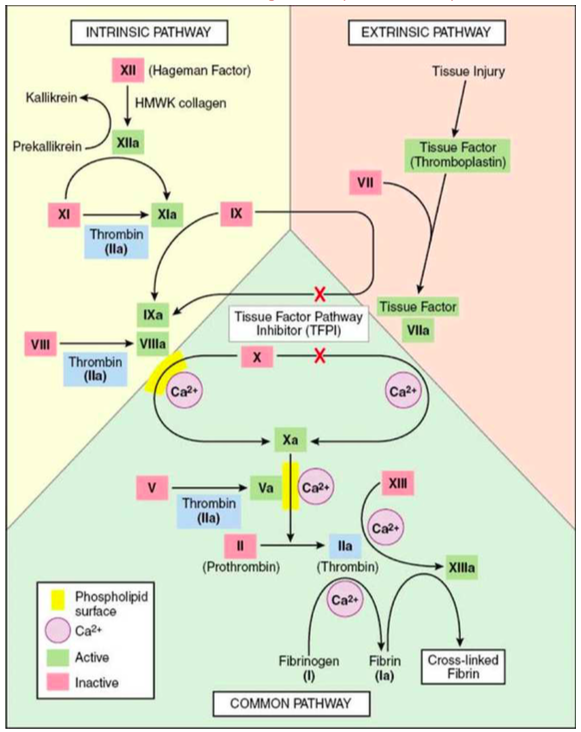
\includegraphics[width=0.8\textwidth]{fig26}
\label{fig26}
\end{figure}

Es reparteixen aix�:
\begin{itemize}
\item Complex I (NADH deshidrogenasa): 7 subunitats
\item Complex III: 1 subunitat
\item Complex IV: 3 subunitats
\item Complex V (ATP sintasa): 2 subunitats. Sense el gradient de protons, aquest enzim �s una ATPasa.
\end{itemize}

\begin{figure}[H]
\centering
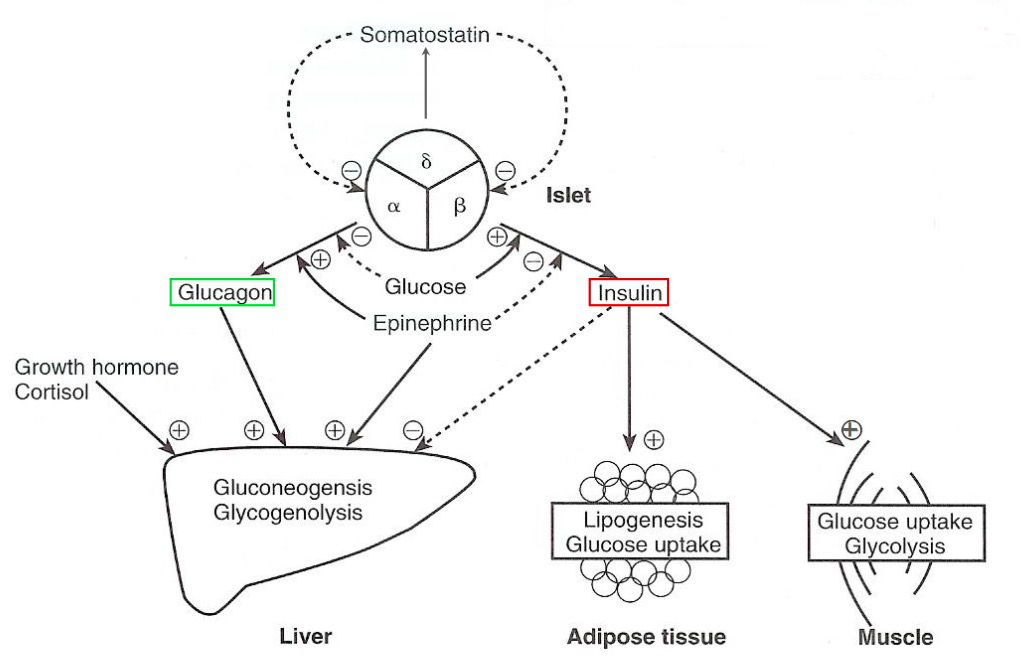
\includegraphics[width=0.6\textwidth]{fig27}
\label{fig27}
\end{figure}

El genoma mitocondrial es coordina amb el genoma nuclear per sintetitzar els complexes mitocondrials sincr�nicament. El mitocondri t� un sistema de traducci� propi. Els ribosomes mitocondrials s�n m�s petits. Els rRNA (12S i 18S) components d'aquests ribosomes estan codificats al genoma mitocondrial. Les prote�nes dels ribosomes mitocondrials estan codificats al genoma nuclear. Els tRNA s�n menys petits i diversos, amb un codi gen�tic diferent.

El D-loop �s una zona no codificant que t� els elements reguladors de la replicaci� i la transcripci�. Les 2 cadenes del genoma mitocondrial s'anomenen H i K (\textit{heavy} i \textit{light}). La que t� pocs gens �s la L i la H cont� molts gens.

El DNA mitocondrial es transcriu en bloc, d�na lloc a un mRNA policistr�nic que es processa i produeix els RNA espec�fics. Es fa un transcrit que comen�a al D-loop i despr�s continua per tota la cadena H. La transcripci� es pot aturar fins a la seq��ncia del tRNA de la Leu. La RNA polimerasa �s diferent que la del genoma nuclear.

Hi ha 2 opinions sobre la finalitzaci� prematura:
\begin{itemize}
\item Factors a l'inici de la transcripci�
\item Factors al final de la transcripci�
\end{itemize}

La replicaci� del DNA mitocondrial va desacoblada a la replicaci� del genoma nuclear. Una c�l�lula proliferativa pot no replicar el DNA mitocondrial i una c�l�lula quiescent pot replicar el DNA mitocondrial. En l'exercici cr�nic, hi ha una replicaci� de DNA mitocondrial al m�scul esquel�tic per refor�ar la cadena respirat�ria. La replicaci� del genoma mitocondrial comen�a al D-loop i es replica nom�s la cadena H fins a una zona reguladora en qu� comen�a la cadena L. Es forma un heterotr�plex: les 2 cadenes mare i un tros de la cadena nova. La DNA polimerasa �s diferent de la nuclear, est� codificada al DNA nuclear i es sintetitza al citoplasma.

\subsection{Mutacions al genoma mitocondrial}
\label{sec:mutacions-al-genoma}
La taxa de mutaci� �s m�s alta que al genoma nuclear. Aix� s'explicaria perqu� el DNA mitocondrial no est� estructurat en cromatina. Es considera que el DNA mitocondrial est� m�s exposat a mut�gens. Al mitocondri es generen moltes ROS, que s�n potents mut�gens. Si la reducci� de l'oxigen �s incompleta, es formen ions super�xid.

Les mutacions podran ser polim�rfiques o patol�giques. La primera seq��ncia que es va obtenir es fa servir de refer�ncia i s'anomena seq��ncia Cambridge. Un problema important �s discriminar la patogenicitat de la mutaci�.

\subsection{Her�ncia del genoma mitocondrial}
\label{sec:herencia-del-genoma}
El DNA mitocondrial no es recombina i �s de transmissi� materna.

La ovella Dolly es va obtenir enucleant un o�cit i introduint el nucli d'una c�l�lula som�tica. S'ent�n que una part del DNA mitocondrial es va transferir de la c�l�lula som�tica a l'o�cit. L'o�cit tindria un sistema de reconeixement i degradaci� selectiva del DNA mitocondrial exogen.

L'her�ncia de la mutaci� no ser� mendeliana. Moltes vegades s�n espont�nies per�.

\begin{figure}[H]
\centering
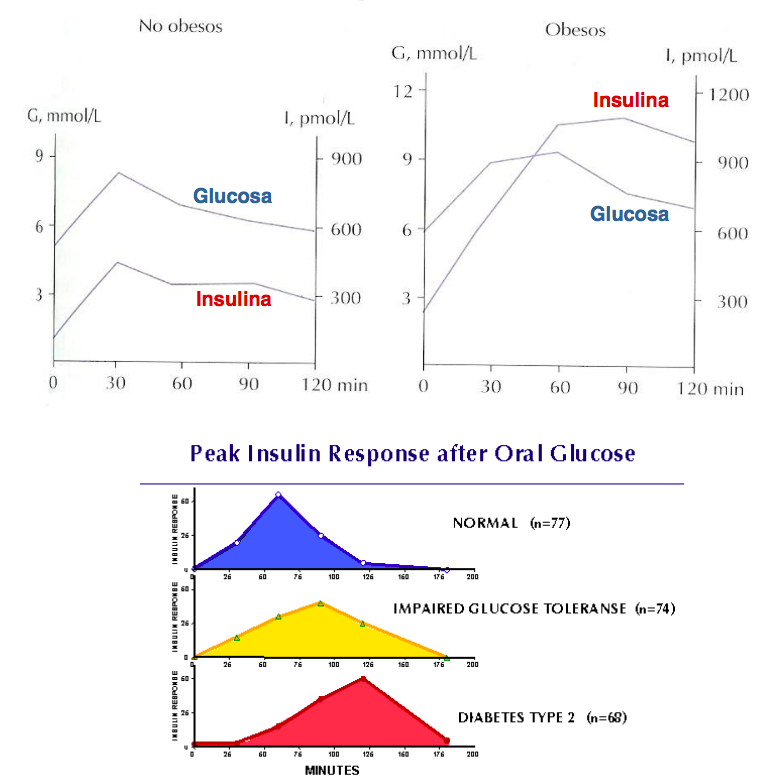
\includegraphics[width=0.8\textwidth]{fig28}
\label{fig28}
\end{figure}

En el pacient poden existir mol�cules de mtDNA sanes i mutades. Quan les seq��ncies de mtDNA s�n id�ntiques hi ha homopl�smia. Les manifestacions polim�rfiques es consideren en homopl�smia.

La heteropl�smia es d�na quan hi ha diferents mol�cules de mtDNA. Es d�na la dada en percentatge.

La heteropl�smia pot presentar difer�ncies entre germans de mare i en funci� del teixit. Les c�l�lules sangu�nies tenen menys grau d'heteropl�smia, les c�l�lules en divisi� tenen menys heteropl�smia. Les dades en sang no s�n informatives i s'ha de fer una bi�psia generalment muscular per diagnosticar la heteropl�smia a nivell molecular.

\begin{figure}[H]
\centering
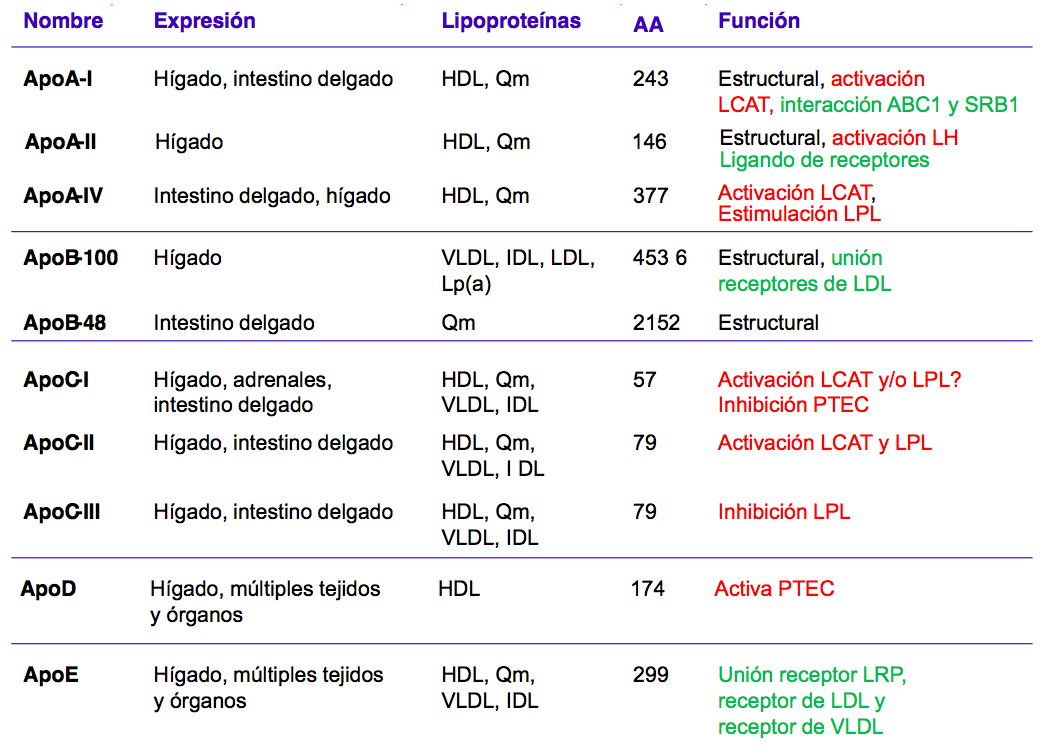
\includegraphics[width=0.8\textwidth]{fig29}
\label{fig29}
\end{figure}

Hi ha un efecte llindar en relaci� als s�mptomes. A partir de cert grau d'heteropl�smia es pot no manifestar cap s�mptoma. Com m�s heteropl�smia hi hagi, m�s greu ser� la malaltia. Amb un 30\% d'heteropl�smia no hi ha cap s�mptoma, p.e.

S�n malalties progressives que empitjoren amb l'edat. Els s�mptomes apareixen de manera molt definida en un �rgan o sistema que �s molt dependent de la funci� mitocondrial per la obtenci� d'energia com el SNC, el m�scul, �rgans sensorials, �rgans endocrins...

Amb el pas del temps, hi ha m�s �rgans afectats. Amb l'edat disminueix l'activitat oxidativa. Els diferents �rgans tenen llindars espec�fics d'activitat oxidativa m�nima per funcionar. Com que amb l'edat va disminuint l'activitat oxidativa, amb el temps s'arriba a superar els llindars d'activitat oxidativa per cada teixit i aix� es van manifestant els s�mptomes progressivament. En funci� del grau d'heteropl�smia, la malaltia es manifestar� abans.

Es considera que l'o�cit t� 100.000 c�pies de mtDNA. Aquest no es replica fins a l'estadi de blastocist. Cada c�l�lula del blastocist t� 1.000 c�pies de mtDNA. Les c�l�lules som�tiques tenen entre 1.000 i 10.000 mol�cules de mtDNA.

\subsection{Malalties mitocondrials}
\label{sec:malalt-mitoc}

Hi ha dificultats per establir un fenotip totalment distintiu (sovint els s�mptomes se solapen amb malalties neuromusculars amb altres or�gens patog�nics). Un diagn�stic fidedigne nom�s �s possible despr�s d'un an�lisi molecular del mtDNA.

Hi ha m�ltiples teixits afectats, sobretot els m�s dependents de la generaci� d'ATP via mitocondrial (cervell, m�scul, �rgans endocrins)... Despr�s dels s�mptomes inicials es desenvolupen fallades als teixits afectats i una disseminaci� dels s�mptomes a altres �rgans i teixits.

Les malalties poden ser per:
\begin{itemize}
\item Deleci� d'un fragment de mtDNA
\item Mutacions puntuals
\item Depleci� mt DNA: Les c�l�lules tenen poc DNA mitocondrial
\end{itemize}

\subsubsection{Malalties per deleci�}
\label{sec:malalt-per-delec}

El s�ndrome de Kearns-Sayre apareix a la inf�ncia avan�ada i es manifesta amb neuropatia i at�xia.

La s�ndrome de Pearson �s de manifestaci� neonatal i es presenta com una an�mia molt greu.

L'oftalmopl�gia progressiva externa �s una dificultat del control de la musculatura al voltant dels ulls. Apareix a la vida adulta i en algunes ocasions pot progressar a miopatia.

Aquests 3 s�ndromes s�n causats per delecions al mtDNA. La gravetat ve determinada pel grau d'heteropl�smia. Els pacients supervivents de Pearson desenvolupen KSS.

La deleci� inclou la zona entre els or�gens de replicaci� del mtDNA. Hi ha qui defensa que les formes delecionades de mtDNA tenen un avantatge sobre les mol�cules de mtDNA intactes. Sembla que l'origen est� en la generaci� d'estructures tipus loop quan es replica el mtDNA. La deleci� pot afectar tRNA.

\begin{figure}[H]
\centering
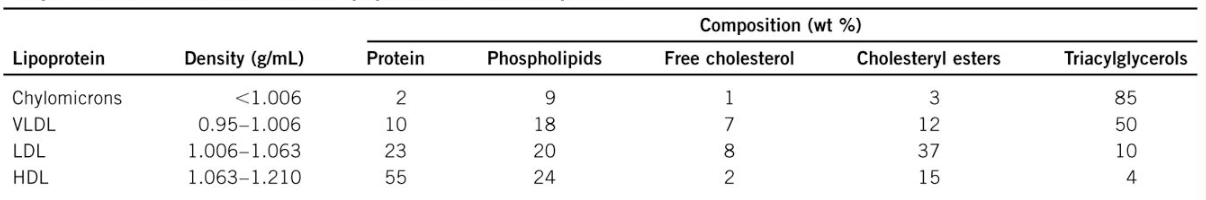
\includegraphics[width=0.8\textwidth]{fig30}
\label{fig30}
\end{figure}

La gravetat de les malalties s'ordenaria S�ndrome de Pearson > KSS > PEO.

\subsubsection{Malalties per mutaci� puntual}
\label{sec:malalt-per-mutac}

\begin{itemize}
\item MELAS (\textit{Myiopathy, stroke-like episodies, lactic acidosis}), degut a lesions focals al cervell al l�bul parito-occipital, acidosi l�ctica i/o RFFs.

\item MERRF (\textit{myoclonic epiplepsy}). Es troba \textit{red ragged fibers} a les fibres musculars. Mioclonus, epil�psia, debilitat muscular i RFF, at�xia cerebel�lar, sordesa i dem�ncia.

\item  NARP \textit{neuropatia, at�xia i retinitis pigmentosa}: Mutaci� puntual a ATP6. At�xia, retinopatia pigment�ria, neuropatia perif�rica i debilitat neurog�nica distal.

\item Hearing loss-ataxia-myoclonus: P�rdua d'o�da sindr�mica, epil�psia miocl�nica, at�xia, miopatia.

\item LHON: P�rdua de visi� central, escotoma gran absolut centrocecal gran, telangiect�sia circumpapil�lar, microangiopatia. LHON �s d'her�ncia materna (abans moltes malalties apareixien \textit{de novo}). Afecta el nervi �ptic. Diferents mutacions causals que afecten els gens ND (complex I de la cadena respirat�ria) al nervi �ptic. La c�l�lula t� adaptacions per viure sense NS.
\end{itemize}

\begin{figure}[H]
\centering
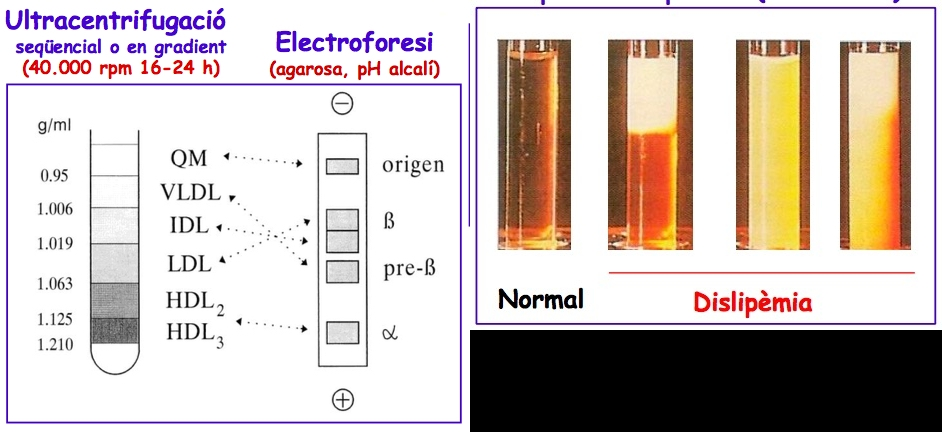
\includegraphics[width=0.8\textwidth]{fig31}
\label{fig31}
\end{figure}

Quan el m�scul es tenyeix amb tricr�mica de Gomori, apareixen fibres vermelles esquin�ades (RRF, \textit{red ragged fibers}) caracter�stiques que s�n visibles al microscopi. Aquest aspecte �s causa de l'acumulaci� dels mitocondris anormals per sota de la membrana plasm�tica de la fibra muscular. Aquests es poden estendre al llarg de la fibra muscular a mesura que augmenta la gravetat de la malaltia. Els agregats mitocondrials causen el contorn de la fibra muscular per convertir-se en irregular, provocant l'aparici� "desigual". A m�s dels m�sculs, el que altres teixits es pot esperar a patir m�s danys causats per un defecte mitocondrial?

La s�ndrome de Lay provoca apoptosi al cervell (encefalopatia necrotitzant). Tenen una mutaci� a ATP6 i m�s heteropl�smia que NARP.

Hi ha altres malalties causades per gens nuclears implicats en el manteniment del DNA mitocondrial i la cadena respirat�ria, com:
\begin{itemize}
\item Gens nuclears que codifiquen complexes de la cadena respirat�ria
\item Gens nuclears que codifiquen prote�nes implicades en l'estructura i assemblatge de complexes de la cadena respirat�ria
\item Gens nuclears que codifiquen prote�nes implicades en la replicaci� i transcripci� del DNA mitocondrial
\end{itemize}

\subsubsection{Deplecions}
La s�ndrome de depleci� del DNA mitocondrial (MDS) es refereix a un grup de trastorns autos�mics recessius que causen que els teixits afectats pateixin d'una depleci� significativa en el DNA mitocondrial. Els s�mptomes poden manifestar-se com miop�tics, hepatop�tics, i/o encefalomiop�tics. Aquests s�ndromes afecten teixits que es troben en el m�scul, el fetge, o tant el m�scul i el cervell, respectivament. La condici� sol ser mortal en la inf�ncia i la infantesa primerenca, encara que alguns han sobreviscut als seus anys d'adolesc�ncia amb la variant miop�tics i alguns han sobreviscut fins a l'edat adulta amb la variant encefalomiop�tica SUCLA2. Actualment no existeix un tractament curatiu per a qualsevol forma de MDS.

Les caracter�stiques de la depleci� s�n:
\begin{itemize}
\item Disminuci� de les c�pies de DNA

\item Her�ncia autos�mica recessiva

\item Gran heterogene�tat cl�nica

\item Associaci� amb mutacions en molts gens: TK2, DGUOK, MPV17, POLG1, C10ORF2, SUCLA2, 	SUCLG1, RRM2B, TYMP.
\end{itemize}

\begin{figure}[H]
\centering
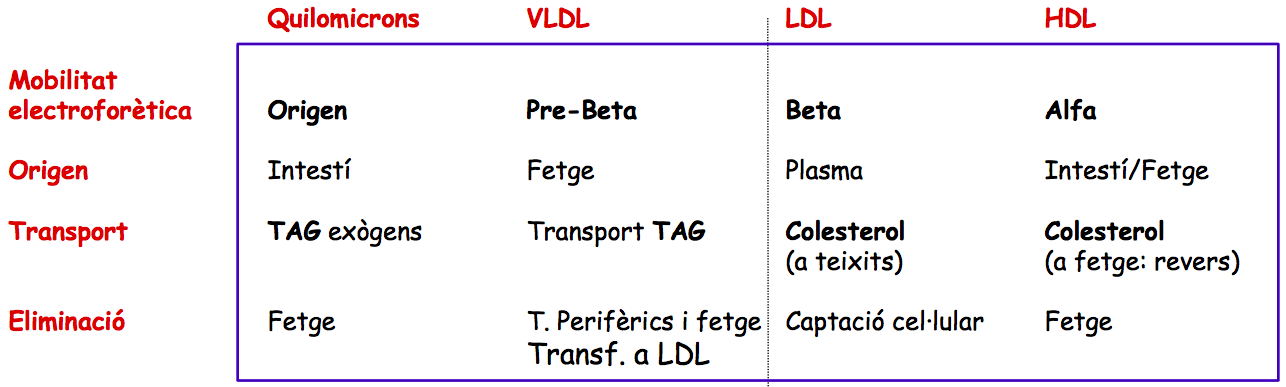
\includegraphics[width=1\textwidth]{fig32}
\label{fig32}
\end{figure}

La forma miop�tica de MDS manifesta s�mptomes dins el primer any de vida, i es diagnostica per la pres�ncia de nivells m�s alts de s�rum de CK, que �s at�pic en altres miopaties mitocondrials. El MDS miop�tic est� fortament correlacionat amb mutacions en el gen TK2, en veure una reducci� de l'activitat TK2 a menys del 32\% en pacients amb MDS trobats amb la mutaci�. Donat que el TK2 juga un paper clau en les rutes de recicaltge mitocondrials de diversos dNTPs, una activitat rebaixada conduiria a menys reciclatge de nucle�tids. Aquesta manca de reciclatge de nucle�tids �s perjudicial ja que els mitocondris no poden sintetitzar completament nous dNTP, i la membrana interna del mitocondri evita que entrin els nucle�tids carregats negativament del citosol. Hi ha una gran variabilitat en el grau de depleci� del mtDNA als teixits afectats, entre el 66 i el 86\%. Es troben RRF al m�scul esquel�tic i defici�ncies en cadenes respirat�ries. Els aspeces cl�nics s�n hipotonia forta, acidosi l�ctica, oftalmopl�gia, lordosi lumbar i dipl�gia facial.

\begin{figure}[H]
\centering
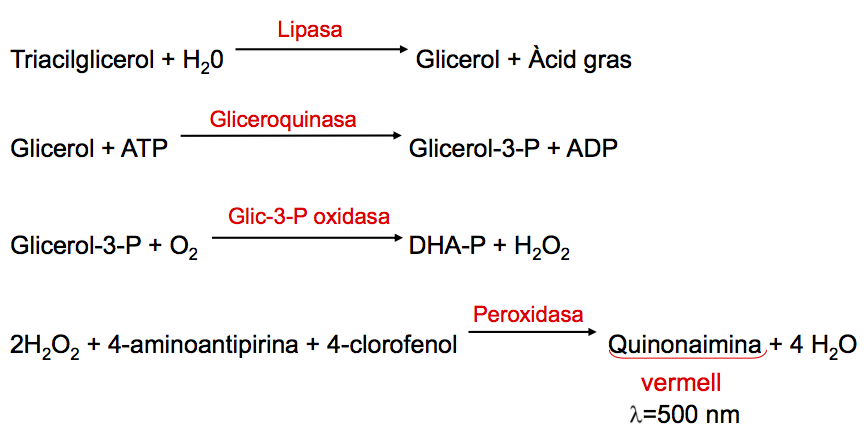
\includegraphics[width=0.8\textwidth]{fig34}
\label{fig34}
\end{figure}

La forma encefalomiop�tica de MDS es caracteritza comunament per retard psicomotor, hipotonia muscular, p�rdua d'audici�, i convulsions generalitzades. Una mutaci� comuna en aquesta forma de MDS �s en el gen SUCLA2, que codifica per a la subunitat $\beta$ de SCS-A. Aquest enzim catalitza la s�ntesi de succinat i coenzim A en succinil-CoA, per� tamb� s'associa amb el complex format per nucle�sid difosfat quinasa (NDPK) en l'�ltim pas de la via de reciclatge de dNTP. Altres formes s'han associat amb mutacions en el gen RRM2B.

La forma hepatop�tiques de MDS consisteixen en l'aparici� de s�mptomes que inclouen hipotonia, hipogluc�mia, v�mits persistents, i la falta de creixement durant el primer any de vida. Les mutacions en tres gens s'han relacionat amb MDS hepatop�tiques : DGUOK, POLG, i Mpv17. DGUOK codifica per la desoxiguanosina cinasa mitocondrial (DGK), que catalitza la fosforilaci� de desoxirribonucle�sids en nucle�tids. POLG codifica per a la subunitat catal�tica $\gamma$A pol, que �s part de la polimerasa de DNA mitocondrial. En aquest cas, la malaltia comen�a en una edat primerenca, t� un mal pron�stic i �s letal durant els primers mesos de vida. La depleci� de mtDNA als teixits afectats �s molt severa (88-99\%) i la defici�ncia de la cadena respirat�ria �s molt greu. Cl�nicament es manifesta com a insufici�ncia hep�tica progressiva, complicacions neurol�giques, hipoglic�mia, hiperlactat�mia.

\begin{figure}[H]
\centering
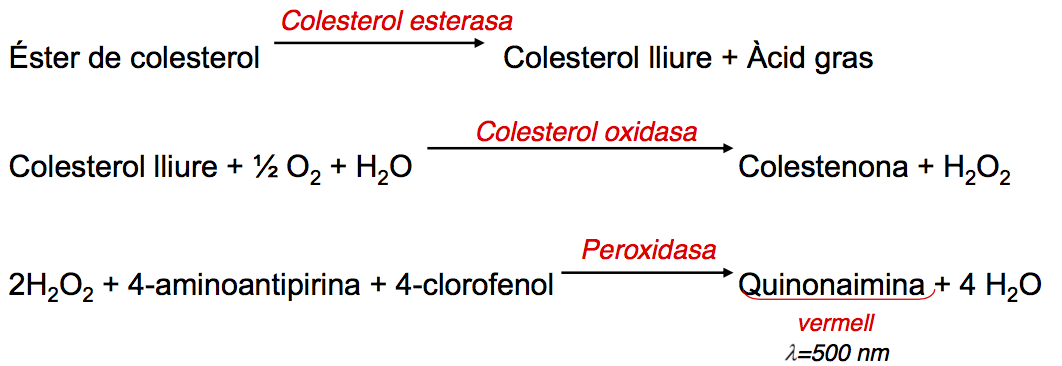
\includegraphics[width=0.8\textwidth]{fig33}
\label{fig33}
\caption{Associaci� entre gens de s�ndrome de depleci� mitocondrial i teixits afectats}
\end{figure}

Algunes MDS s'associen amb mutacions som�tiques al mtDNA, com el MNGIE (\textit{Mitochondrial neurogastrointestinal encephalopathy syndrom}).

La s�ndrome d'encefalopatia neurogastrointestinal mitocondrial (MNGIE) �s un trastorn gen�tic autos�mic recessiu poc freq�ent que generalment apareix entre la segona i la cinquena d�cada de la vida. A difer�ncia de les usuals malalties mitocondrials, que s�n causades per mutacions en l'DNA mitocondrial (DNAmt), la MNGIE �s causada per mutacions en el gen TYMP (localitzat al cromosoma 22q13.32), el qual �s codificat per l'anomenat enzim timidina fosforilasa. Una de les formes secund�ries d'aquesta s�ndrome s'anomena MNGIE sense leucoencefalopatia i pot �sser causada per mutacions en el gen POLG.

Al voltant de 50 mutacions en el gen TYMP han estat identificades en persones amb la s�ndrome de MNGIE. Les mutacions en el TYMP redueixen notablement o eliminen l'activitat de la timidina fosforilasa. L'escassetat d'aquest enzim permet que la timidina s'acumuli al cos en grans quantitats i un exc�s d'aquest subst�ncia �s perjudicial per al DNAmt, ja que altera el seu funcionament habitual (manteniment i reparaci�). Conseg�entment, les mutacions es poden anar acumulant a l'interior del DNAmt causant-li inestabilitat i tamb� pot ser que els mitocondris continguin menys DNAmt de l'habitual. Tots aquests canvis gen�tics alteren el funcionament mitocondrial normal. Malgrat saber que les anomalies del DNAmt emmarquen els problemes digestius i neurol�gics caracter�stics de la s�ndrome MNGIE, avui en dia encara es desconeix com el mitocondri defectu�s causa els trets caracter�stics espec�fics propis de la malaltia.

La MNGIE �s un trastorn autos�mic recessiu (�s a dir, no est� lligada al sexe i per tal que es manifesti cal heretar els dos al�lels mutants), per tant els progenitors han de ser com a m�nim portadors de l'al�lel mutant; els heterozigots no presenten cap s�mptoma. Els medicaments que interfereixen amb la funci� mitocondrial s'han d'evitar tant com sigui possible i utilitzar amb precauci� aquells que es metabolitzin al fetge.

\subsection{Tractament de les malalties mitocondrials}
\label{sec:tractament-de-les}
Hi ha diferents estrat�gies:
\begin{itemize}
\item \textbf{Ter�pia pal�liativa:} Inclou f�rmacs anticonvulsius, control de les alteracions endocrines i procediments quir�rgics.

\item \textbf{Eliminaci� de metab�lits nocius:} Principalment el lactat de l'acidosi l�ctica, per� tamb� timidina en pacients MNGIE.

\item \textbf{Administraci� d'acceptors d'electrons:} Per evitar alguns components de la cadena respirat�ria.

\item \textbf{Administraci� de metab�lits i cofactors:} �s la base de la ter�pia actual. Inclou components de la cadena respirat�ria i altres com L-carnitina o CoQ10 (ubiquinona).

\item \textbf{Scavengers de ROS:} Tant en malalties mitocondrials prim�ries com en malalties neurodegeneratives causades directa o indirectament per una disfunci� mitocondrial.
\end{itemize}

Hi ha estrat�gies de FIV per trasplantar els mitocondris d'una donant sana:
\begin{figure}[H]
\centering
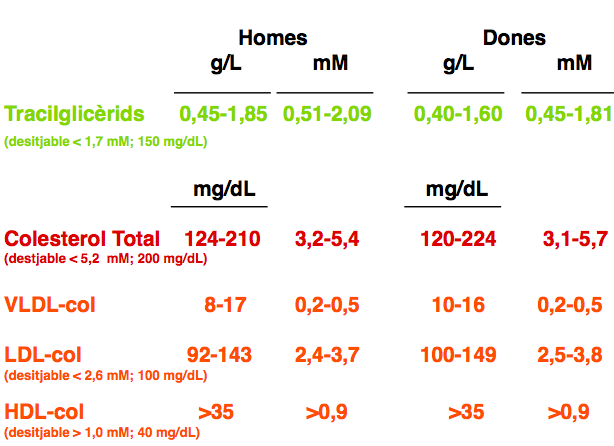
\includegraphics[width=0.8\textwidth]{fig35}
\label{fig35}
\end{figure}

El tractament amb antiretrovirals causa una depleci� del mtDNA, el que acaba en una lipodistr�fia adquirida en pacients amb SIDA. La lipodistr�fia adquirida es caracteritza per una p�rdua severa de teixit adip�s perif�ric per� amb una adipositat central. Els pacients tenen hipertriglicerid�mia, hipercolesterol�mia, acidosi l�ctica, resist�ncia a la insulina i diabetis de tipus 2. Es creu que �s degut a que els an�legs de nucle�sids usats pel tractament del VIH inhibeixen la DNA polimerasa mitocondrial.

%------------------------------------------------------------------------------
% Tema 5. Hemost�sia i coagulaci�
%------------------------------------------------------------------------------
\newpage
%------------------------------------------------------------------------------
% Tema 5. Genètica de la obesitat
%------------------------------------------------------------------------------
\section{Genètica de la obesitat monogènica}
\label{sec:genetica-de-la}

\subsection{Obesitat monogènica}
\label{subsec:obesitat-monogenica}
Les nenes deficients en leptina tenen problemes de maduració sexual i per tant de fertilitat.

Els pacients deficients en MC4R (receptor de melanocortina), que són heterozigots per la mutació. Presenta obesitat a la infància, hiperfàgia, hiperinsulinèmia.

Hi ha 2 tipus de pèptids que controlen la sacietat quan senyalitzen a l'hipotàlem:
\begin{itemize}
\item Orexigènics Inhibits per la leptina
\item Anorexigènics: Estimulats per la leptina. El gen de la POMC quan s'expressa genera un polipèptid de 31 kDa, que en funció de les cèl·lules on s'expressa la proteïna es trenca en diferents fragments que seran els que tenen l'activitat biològica. Aquests fragments poden ser la ACTH, alpha-MSH... alpha-MSH atura la gana, interaccionant amb un receptor hipotalàmic. Quan el nen té dèficits en POMC, es poden donar agonistes pel receptor hipotalàmic.
\end{itemize}

\subsection{Obesitat multifactorial}
\label{subsec:obes-mult}

% tipus d'estudi per identificar gens de susceptibilitat

El gen FTO té una variant que s'associa molt potentment a un BMI alt. En canvi, variants polimòrfiques de la leptina no tenen associació amb la obesitat. BDNF fa de connexió entre l'hipotàlem i l'escorça per generar la sensació conscient de gana/sacietat.

FTO se sabia que tenia un NLS, un domini de demetilasa. FTO es troba en una regió genòmica amb clústers d'IRX (iroguis-related). Introns del FTO regulen els enhancers del gen IRX; el grau d'interacció condiciona l'expressió d'IRX3. IRX3 re demetilasagula la despesa energètica. Els al·lels FTO de risc per obesitat que quan interaccionen amb IRX3 augmenten l'expressió d'IRX3, i IRX3 disminueix la despesa energètica.

%------------------------------------------------------------------------------
% Tema 6. Hemoglobina i ferro
%------------------------------------------------------------------------------
\newpage
%------------------------------------------------------------------------------
% Tema 6. Hemoglobina i ferro
%------------------------------------------------------------------------------
\section{Hemoglobina i ferro}

\subsection{La hemoglobina}
La hemoglobina �s una prote�na globular que dona la coloraci� vermella
de la sang. Responsable del transport de \ch{O2}. T� un pes de  64,45
kDa.

Els nivells normals s�n de 16g/100 mL en homes i de 14g/100 mL en les dones.

Un home de 70 kg t� 900 g d'hemoglobina. El bescanvi d'hemoglobina �s
de 0,3 g/h (sintetitzats i destru�ts).

Classificaci� de les malalties relacionades amb la hemoglobina:
\begin{itemize}
\item Reaccions de l'hemoglobina
  \begin{itemize}
  \item Metahemoglobin�mia heredit�ria
  \end{itemize}

\item S�ntesi de la globina
  \begin{itemize}
  \item Hemoglobinopaties estructurals
    \begin{itemize}
    \item An�mies drepanoc�tiques 
    \item Metahemoglobin�mia cong�nita
    \item Eritrocitosis (alterada afinitat per O2)
    \end{itemize}
  \item Talass�mies (hemoglobines alterades)
    \begin{itemize}
    \item  $\alpha$-talass�mies
    \item $\beta$-talass�mies
    \end{itemize}
  \end{itemize}

\item S�ntesi i degradaci� del grup hemo
  \begin{itemize}
  \item Porfiries agudes
    \begin{itemize}
    \item Porf�ria aguda intermitent 
    \item Coproporf�ria heredit�ria
    \item Porf�ria variegata
   \end{itemize}
  \item Porf�ries no agudes
    \begin{itemize}
    \item Porf�ria eritrohep�tica (eritropoi�tica) 
    \item Porf�ria eritropoi�tica cong�nita
    \item Porf�ria cong�nita (Intoxicaci� per plom)
    \end{itemize}
  \end{itemize}

\item Alteracions del metabolisme del ferro
  \begin{itemize}
  \item An�mia ferrop�nica (manca de ferro)
    \begin{itemize}
    \item P�rdua cr�nica de sang
    \item Ingesta inadequada de ferro
    \end{itemize}
  \item An�mia siderobl�stica (mala utilitzaci� del ferro)
  \item Hemocromatosis (sobrec�rrega de ferro)
  \end{itemize}
\end{itemize}

\subsubsection{Estructura}
Hi ha 6 tipus de globines, que en la seva combinat�ria generen els
diferents tipus d'hemoglobina que trobem en humans. Aquests tipus s�n:
$\alpha$, $\beta$, $\gamma$, $\delta$, $\epsilon$, $\zeta$.

La hemoglobina �s un heterotetr�mer $\alpha_2\beta_2$ en adults. Presenta
cooperativitat amb l'oxigen. Tamb� t� al�losterisme amb el
2,3-difosfoglicerat, un intermediari de la glic�lisi que nom�s es
troba en eritr�cits. Aix� facilita l'alliberaci� d'oxigen als
teixits.

Es sintetitza als reticul�cits (eritr�cits immadurs).

La hemoglobina presenta diferents subunitats segons l'estadi de
desenvolupament de l'individu:
\begin{itemize}
\item Adult:
  \begin{itemize}
  \item Hemoglobina A1 ($\alpha_2\beta_2$)
  \item Hemoglobina A2 ($\alpha_2\delta_2$)
  \end{itemize}

\item Fetal: Cadenes $\alpha_2\gamma_2$

\item Embri�:
  \begin{itemize}
  \item Grower I: $\zeta_2\epsilon_2$
  \item Grower II: $\alpha_2\epsilon_2$
  \item Portland: $\zeta_2\gamma_2$
  \end{itemize}
\end{itemize}

Hi ha 2 loci d' $\alpha$-globina al cromosoma 16 i un locus de $\beta$-globina
al cromosoma 11.

\subsection{Trastorns deguts a reaccions de l'hemoglobina}
La carboxihemoglobina presenta menys afinitat per l'hemoglobina.

\begin{figure}[H]
  \centering
  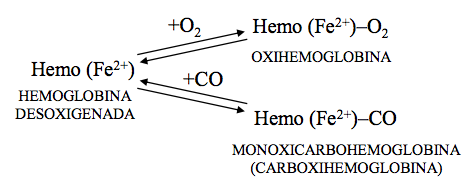
\includegraphics[width=0.5\textwidth]{fig5}
\end{figure}

Molt f�rmacs o agents oxidants poden provocar la formaci� de
metahemoglobina (amb \ch{Fe3+}), que mitjan�ant la NADH-metahemoglobina
reductasa la torna a reduir.

\begin{figure}[H]
  \centering
  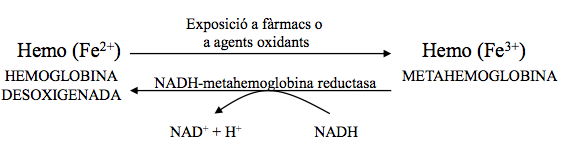
\includegraphics[width=0.5\textwidth]{fig6}
\end{figure}

La metahemoglobin�mia heredit�ria �s una defici�ncia en NADH-metahemoglobina
reductasa. El Fe del hemo s'oxida en 25 \% a \ch{Fe3+} Es manifesta amb
cianosi (coloraci� fosca a la pell). Es tracta amb f�rmacs que
redueixin lametahemoglobina. �s una malaltia
molt greu.

\subsection{Trastorns a la s�ntesi de la globina}
\subsubsection{Hemoglobinopaties estructurals}
Les mutacions perjudicials desapareixen, per� les altres poden sobreviure
(els heterozigots resisteixen m�s que els homozigots). Algunes
mutacions s�n in�cues.

\paragraph{Hemoglobina S. An�mia drepanoc�tica} \hfill \\
Es d�na un canvi d'amino�cid Glu->Val a la cadena beta. �s insoluble a baixes pressions
de \ch{O2}. Els gl�buls vermells presenten una morfologia
falciforme. Quan est� desoxigenada, la hemoglobina es polimeritza i es
deformen els eritr�cits. Els heterozigots  presenten poques vegades s�mptomes greus

Es va originar a Africa i confereix resist�ncia a la mal�ria. La
presenten un 40 \% de la poblaci� africana i un 10\% dels negres
americans.

La Hb pot polimeritzar formant fibres de 3000 \AA{}. Hi ha cicles
successius de forma de fal� i normal. La forma de fal� es trenca als
capil�lars per falta de flexibilitat. L'an�mia s'agreuja amb oxidants.

Altes concentracions d'HbS d'afinitat baixa per \ch{O2} no donen cap
problema fins l'administraci� d'un agent oxidant.

L'an�mia �s menys severa si �s dependent d'HbF. Els pacients tendeixen
a augmentar la proporci� d'HbF en l'adult. Els homozigots d'Orient
Mitj� s�n asimptom�tics ja que tenen un 18\% d'HbF.

El diagn�stic es fa per electroforesi de la hemoglobina o per examen
microsc�pic d'un frotis de sang.

Encara no hi ha tractament, encara que hi ha f�rmcs en estudi. La
profilaxi es basa en una bona nutrici� i higiene, contra la
mal�ria. En cas d'infecci�, s'actua sobre l'agent infecci�s. Si es fa
una transfusi� quan es dona la primoquina ja que �s oxidant i es pot
agreujar l'an�mia.

\paragraph{Hemoglobinopaties inestables} \hfill \\
S'han descrit m�s de 100 hemoglobinopaties. Es produeix la formaci� de
cossos d'inclusi� intraeritroc�tics (cossos de Heinz), que s�n
precipitacions d'hemoglobina. Consisteix en una s�rie de petites
granulacions que se situen a la perif�ria dels hematies. Es produeix
en malalties cong�nites.

\begin{figure}[H]
  \centering
  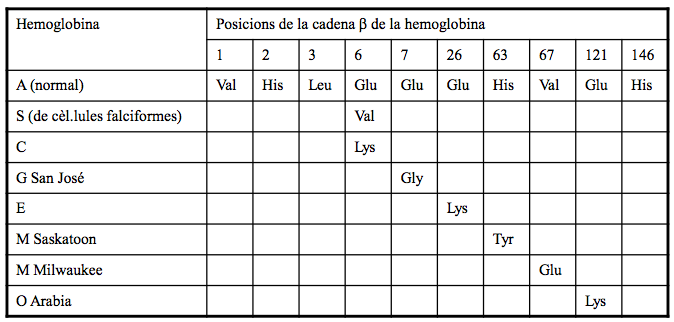
\includegraphics[width=0.8\textwidth]{fig7}
  \caption{Composici� parcial en amino�cids en la cadena $\beta$ humana
    normal i algunes hemoglobines amb cadenes $\beta$ anormals. Altres
    hemoglobines tenen cadenes $\alpha$ anormals.}
  \label{fig:fig7}
\end{figure}

\paragraph{Eritrocitosis} \hfill \\
Alteraci� en l'afinitat per \ch{O2}. En casos lleus no requereix
farmacologia. L'afinitat �s m�s alta degut a canvis que eviten la uni�
de 2,3-difosfoglicerat. Es produeix una hip�xia lleu (augment d'eritr�cits).

\subsubsection{Talass�mies}

%------------------------------------------------------------------------------
% Tema 7. Enzimologia cl�nica
%------------------------------------------------------------------------------
\newpage
%------------------------------------------------------------------------------
% Tema 7. Enzimologia cl�nica
%------------------------------------------------------------------------------
\section{Enzimologia cl�nica}

\subsection{Enzims}
L'enzimologia cl�nica �s un conjunt de t�cniques destinades a detectar
la pres�ncia i a quantificar l'activitat d'enzims en mostres biol�giques:
\begin{itemize}
\item Pres�ncia d'enzims que no es trobin normalement en
  concentracions significatives
\item Variacions en els nivells d'enzims que poden trobar-se
  normalment en mostres biol�giques
\item Isoenzims (formes diferents d'un enzim)
\end{itemize}

Es poden utilitzar enzims com a reactius espec�fics per quantificar la
concentraci� de metab�lits.

Un enzim �s un biocatalitzador proteic. Es localitzen en tots els
teixits corporals. Es determinen mitjan�ant la reacci� enzim�tica. Un
holoenzim est� format per un apoenzim (porci� proteica) i coenzim
(porci� no proteica no sempre necess�ria). L'activitat enzim�tica es
pot veure redu�da si no hi ha apoenzim o coenzim.

Els enzims tenen destrucci� citoplasm�tica o mitocondrial. A la
circulaci� es poden eliminar per catabolisme que alliberar� amino�cids
i grups prost�tics per la s�ntesi de noves prote�nes i/o enzims.

Tots els enzims s�rics tenen un origen cel�lular. Apareixen al s�rum
com a conseq��ncia d'una lesi� cel�lular (en petites quantitats de la
degradaci� cel�lular). Les activitats enzim�tiques del s�rum s�n �tils
pel diagn�stic de malalties particulars o anomalies fisiol�giques.

Quan les c�l�lules estan en proliferaci�, augmenta la s�ntesi d'enzims
i s'atura el seu catabolsime. En l'estat d'inactivaci�, hi ha un
descens de la s�ntesi d'enzims i augmenta la seva degradaci� degut a
la car�ncia de cofactors. 

Els enzims difonen a la limfa, passen a la sang on s'inactiven (p�rdua
de grups prost�tics, canvis conformacionals) i es catabolitzen. Els
enzims es destrueixen en fag�cits, melsa, endotelials, c�l�lules sangu�nies.

L'�s de certs enzims per diagnosticar malalties �s per circumst�ncies
hist�riques. No �s normal que un enzim que funciona sigui substitu�t
per un altre, a no ser que la utilitat diagn�stica sigui molt millor.

\subsubsection{Lesi� cel�lular}
Hi ha enzims i metab�lits intracel�lulars i extracel�lulars en una
situaci� normal. Si hi ha una lesi� cel�lular, es detecten enzims i
metab�lits intracel�lulars a la sang.

Els enzims intracel�lulars poden apar�ixer al plasma degut als
processos normals de recanvi cel�lular. L'increment dels enzims pot
ser degut a la lesi� cel�lular o a l'augment de la proliferaci�.

\subsubsection{Mesura de la concentraci� dels enzims}
\begin{itemize}
\item \textbf{Concentraci� de massa:} Quantitat de l'enzim.
\item \textbf{Concentraci� catal�tica:} Activitat de l'enzim. �s el
  m�s usat. Es pot expressar com a:
  \begin{itemize}
  \item Activitat enzim�tica: Quantitat d'enzim que transforma un
    micromol de substrat per minut a 25�C. Es poden fer servir UI o katals.
  \item Activitat espec�fica: Unitats de l'enzim per mil�ligram de prote�na
  \item Activitat molecular o molar: N�mero de mol�cules de substrat
    trasformades per minut per
una sola mol�cula d'enzim
  \end{itemize}
\item Concentraci� d'isoformes: Permet discriminar el teixit d'origen.
\end{itemize}

L'activitat enzim�tica pot variar degut a la temperatura, pH,
concentraci� de substrat, for�a i�nica... La prova s'ha d'adequar a
les concentracions �ptimes de l'enzim.

\subsubsection{Distribuci� cel�lular dels enzims}
% Taula
\begin{table}[H]
  \centering
  
  \caption{Localitzaci� subcel�lular d'enzims amb import�ncia cl�nica}
  \label{tab:enzims}
\end{table}

La pres�ncia d'enzims mitocondrials en s�rum �s indicatiu de dany greu.

La detecci� d'una isoforma permet fer un diagn�stic m�s prec�s. Es
poden detectar per:
\begin{itemize}
\item Difer�ncia de c�rrega neta (cromatografia, electroforesi,
  isoelectroenfocament)
\item Acci� selectiva de determinades subst�ncies (inhibici�
  selectiva)
\item T�cniques immunol�giques (immunoinhibici�, enzimimmunoassaig)
\end{itemize}

Poden alliberar-se els enzims encara que no hi hagi necrosi h�stica
(augment de la permeabilitat de les membranes) als teixits. Exemple:
delirium tremens.

La fosfatasa alcalina �s un marcador per malalties hepatobiliars. En
canvi, hi ha altres enzims m�s bons com la leucinaminopeptidasa o la
5'-nucleotidasa.

Un altre exemple �s la GPT (hepatopatia) que no ha estat substitu�da
per la ornitin-carbamo�l-transferasa o iditol-deshidrogenasa.

\subsubsection{Inter�s diagn�stic dels enzims}
Les an�lisis enzim�tiques representen fins un 20\% de les proves
bioqu�miques. Els laboratoris de bioqu�mica cl�nica poden determinar
entre 12-15 enzims diferents.

Actualment s'han determinat me??s de 60 enzims en s�rum, dels quals:
\begin{itemize}
\item Alguns es determinen habitualment al laboratori
\item Alguns s�n reflex de diverses malalties, per� no es determinen
  degut a la seva dificultat
\item Alguns s�n importants a nivell de recerca, i nom�s es determinen
  en situacions cl�niques especials
\end{itemize}

% posar taula

\subsection{Estrat�gies bioqu�miques per l'estudi cl�nic del
  metabolisme}

Els enzims es poden estudiar de diferents maneres:
\begin{enumerate}
\item Determinaci� de la concentraci� de metab�lits en l�quids i
  teixits biol�gics
\item Determinaci� d'activitats enzim�tiques en l�quids i teixits
  biol�gics
\item Diferenciaci� de les formes isoenzim�tiques
\item An�lisi de la resposta metab�lica en front proves diagn�stiques
  espec�fiques
\end{enumerate}

\subsubsection{Cin�tica de les reaccions enzim�tiques monosubstrat}
Si:
\begin{itemize}
\item L'espectrofot�metre absorbeix el substrat, l'absorb�ncia
  disminuir� en funci� del temps.
\item L'espectrofot�metre absorbeix el producte, l'absorb�ncia
  augmentar� en funci� del temps.
\end{itemize}

S'ha d'escollir la longitud d'ona on es distingeixi l'absorci� del
substracte de la del producte.

\subsubsection{Procediments per a mesurar la velocitat de
  transformacio??}

Hi ha 2 tipus:
\begin{enumerate}
\item \textbf{Procediments discontinus:}
  \begin{enumerate}
  \item A un punt.- Es mesura l???absorba??ncia de la mostra i de un blanc
    al cap d???un temps determinat.
    \begin{equation}
      \label{eq:1}
      v = \frac{A_t-A_{Blanc}}{t}
    \end{equation}
  \item A dos punts.- Es mesuren 2 absorba??ncies (A1, A2) a dos temps
    (t1, t2).
    \begin{equation}
      \label{eq:2}
      v = \frac{A_2-A_1}{t_2-t_1}
    \end{equation}
  \item A tres o me??s punts.- Es mesura l???absorba??ncia a diversos valors
    de temps (mesurar dos punts pot ser inexacte).
    \begin{equation}
      \label{eq:3}
      v = \frac{\Delta A}{\Delta t}
    \end{equation}
  \end{enumerate}

\item \textbf{Procediments continus:} Es mesura l???absorba??ncia
  continuament durant un temps determinat.
  \begin{equation}
    \label{eq:4}
    v = \frac{d A}{d t} 
  \end{equation}
\end{enumerate}

\subsubsection{Aplicacio?? de te??cniques enzima??tiques combinades}
La concentraci� dels enzims �s molt baixa (nmol) i per tant es mesura
la seva activitat (o b� s'aplica immunoan�lisi).

Hi ha 3 fases de l'activitat enzim�tica:
\begin{enumerate}
\item Periode de lante??ncia. La velocitat va augmentant progressivament.
\item Estat estacionari. La velocitat e??s proporcional a la
  concentracio?? de l???enzim. 
\item Fase final.- la velocitat disminueix progressivament e??s on es fa
  l'an�lisi)
\end{enumerate}

La malalt deshidrogenasa t� concentracions molt baixes, per tant
s'aplica a reaccions acoblades. Es mira l'activitat de l'enzim
anterior o posterior.

% Exemple de diap 13.

\subsubsection{Procediment general d'an�lisi per espectrofotometria
  visible o UV}
L'espectrosc�pia estudia els sistemes mitjan�ant la seva interacci�
amb les radiacions electromagn�tiques. Un sistema �s un conjunt de
part�cules materials (�toms, mol�cules).
\begin{itemize}
\item Absorci�
\item Emissi�
\item Difracci�
\end{itemize}

L'espectrometria d'absorci� molecular UV-visible �s molt utilitzada en
cl�nica. Estudia l'absorci� de la radiaci� magn�tica ultravioleta i
visible. Permet mesurar la concentraci� d'una subst�ncia.

L'espectre electromagn�tic �s el conjunt de totes les longituds d'ona.

En un laboratori cl�nic s'utilitza amb m�s freq��ncia les regions
visible i ultraviolada.

Els espectrofot�metres poden ser de:
\begin{itemize}
\item Feix simple: Primer es posa el blanc com a refer�ncia i despr�s
  la mostra.
\item Feix doble: Detecta el blanc i la mostra alhora.
\end{itemize}

\subsection{Enzims marcadors habituals en enzimologia cl�nica}


%------------------------------------------------------------------------------
% Tema 8. Disfuncions del metabolisme gluc�dic
%------------------------------------------------------------------------------
\newpage
%------------------------------------------------------------------------------
% Tema 8. Disfuncions del metabolisme gluc�dic
%------------------------------------------------------------------------------
\section{Disfuncions del metabolisme gluc�dic}
\label{sec:disf-del-metab}

\subsection{Regulaci� de la concentraci� de la glucosa sangu�nia}
\label{sec:regulacio-de-la}
% Recordatori insulina/glucag�

Els nivells normals de glucosa en sang s�n de 3,89-5,83 mmols/L
(70-105 mg/dL).

\subsection{Hipergluc�mies}
\label{sec:hiperglucemies}
Hi ha 4 tipus d'hipergluc�mia:
\begin{itemize}
\item \textbf{Diabetis tipus 1:} Hipergluc�mia de manera abrupta. Els pacients
  necessiten insulina per sobreviure.
\item \textbf{Diabetis tipus 2:} Progressi� gradual i la insulina no acostuma a
  ser necess�ria pel tractament.
\item \textbf{Altres tipus espec�fics}
\item \textbf{Diabetis gestacional:} Es produeix en l'�ltim ter� de la
  gestaci�. Normalment acaba despr�s del part per� en alguns casos el
  quadre hipergluc�mic continua.
\end{itemize}

Hi ha 2 subgrups poblacionals en risc de diabetis:
\begin{itemize}
\item Intoler�ncia a la glucosa: 2h despr�s de la ingesta de 75 de
  glucosa, els nivells de glucosa es troben entre 140 i 199 mg/dL.

\item Disfunci� de la glucosa en dejuni: La glucosa es troba entre 100
  i 125 mg/dL.
\end{itemize}

Hi ha un marcador circulant usat per monitoritzar els diab�tics que �s
la hemoglobina $A_{1c}$. L'hemoglobina incorpora glucosa
espont�niament a la seva estructura i s�n un reflex dels nivells
circulants de glucosa. Aquesta hemoglobina t� una vida mitja llarga.

Els nous criteris diagn�stics de la diabetis s�n:
\begin{itemize}
\item S�mptomes de diabetis m�s una concentraci� casual (no en dejuni)
  de glucosa superior a 200 mg/dL.
\item Glucosa en plasma despr�s d'un dejuni m�nim de 8 hores superiors
  a 126 mg/dL.
\item Gluc�mia superior a 200 mg/dL despr�s de 2 hores del test de
  toler�ncia oral de glucosa.
\item Nivells Hb$A_{1c}$ superiors a 6,5\%.
\end{itemize}

% Taula comparativa

\subsubsection{Alteracions metab�liques}
\label{sec:alter-metab}
Augmenten els nivells de TAG ja que la LPL �s sensible a
insulina. Cetoacidosi.

El fetge activa la gluconeog�nesi i la glicogen�lisi, fet que augmenta
la glucosa circulant.

Tamb� augmenta la cetog�nesi, degut a la beta oxidaci� dels �cids
grassos alliberats del teixit adip�s, que est� fent lip�lisi. Els
acetilCoA no es poden utilitzar al cicle de Krebs ja que els
intermediaris estan dirigits a la GNG. Els cossos cet�nics
proporcionen energia a altres teixits per� provoquen cetoacidosi
(acidosi metab�lica).

\subsubsection{Complicacions}
\label{sec:complicacions}
Alteracions de la microvasculatura i la macrovasculatura. Els vasos es
malmeten i generen gangrena sobretot als peus.

Hi ha neuropatia.

Tamb� hi pot haver retinopatia diab�tica.

Els ronyons tamb� pateixen un dany. La glucosa �s un osm�lit, i com
que la concentraci� �s tant alta no es pot reabsorbir a nivell
tubular. La glucosa malmet els glom�ruls renals. L'epiteli fenestrat
presenta c�rregues negatives i impedeix el pas de prote�nes. La
glucosa alta fa que els glom�ruls siguin m�s permeables i que a la
orina hi hagi m�s prote�nes, majorit�riament alb�mina perqu� �s la
prote�na m�s abundant del plasma i t� un pes de 65 kDa, l�mit de mida
per filtrar als glom�ruls (60 kDa).

Tamb� hi ha m�s risc de patir aterosclerosi. Sembla que estar
relacionada amb un proc�s de glicosilaci� de la superf�cie de les
lipoprote�nes.

\subsection{Par�metres cl�nics}
\label{sec:parametres-clinics}

\subsubsection{Glucosa}
\label{sec:glucosa}
El m�tode de l'ortotolu�dina consisteix que en medi �cid, la glucosa
reacciona amb amines arom�tiques i genera color. Un altre m�tode, el
de Benedict est� basat en la reducci� del Cu (usat en tires reactives
per la orina).

El m�tode de refer�ncia �s el m�tode que han de tenir tots els
laboratoris i poder avaluar la qualitat inter-laboratoris. Per la
glucosa, �s el m�tode basat en la hexoquinasa i la
glucosa-6-P-deshidrogenasa. La reacci� genera NADPH, que es pot
mesurar a 340 nm.

Hi pot haver diferents fonts de variabilitat:
\begin{itemize}
\item Sang/S�rum o plasma. Normalment no s'usa sang total, ja que els
  eritr�cits consumeixen glucosa i els valors sortirien m�s baixos
  dels reals.
\item La concentraci� arterial �s superior a la venosa.
\item L'edat, els f�rmacs (corticoides i di�r�tics) augmenten la
  glucosa.
\end{itemize}

Diferents precaucions que s'han de prendre:
\begin{itemize}
\item No ha de ser sang total (eritr�cits contenen < [glc])
\item Cal ser r�pids per evitar metabolisme eritrocitari
\item Desproteinitzaci� pr�via per evitar interfer�ncies
\item Estabilitat 8h a 25�C ??? 72h a 4�C
\end{itemize}

\subsubsection{Sobrec�rrega oral de glucosa (SOG)}
\label{sec:sobrecarrega-oral-de}
Si surt un valor alt de gluc�mia, es repeteix l'anal�tica. Si torna a
sortir hipergluc�mia es practica un test de sobrec�rrega oral de
glucosa o test de toler�ncia oral a la glucosa. Aquest test es
realitza en 4 situacions:
\begin{enumerate}
\item Diabetis gestacional
\item Intoler�ncia a la glucosa (IGT)
\item Neuropaties, nefropaties o retinopaties. En casos que la
  gluc�mia sigui inferior a 140 mg/dL (7,7 mM).
\item Epidemiologia
\end{enumerate}

El test consisteix en ingerir 75g de glucosa pels adults i 1,75 g de
glucosa/kg en nadons i nens. S'extreu sang a $t_0$ en dejuni i en
situaci� normal. Cada cert temps es mesura la gluc�mia i s'avalua
l'evoluci� de la gluc�mia. Els resultats poden ser:
\begin{enumerate}
\item Normal: Pic abrupte a 30 minuts fins que a les 2h es normalitza
  la gluc�mia.
\item Diabetis: Fa un pic abrupte a 30 min i despr�s un  plateau m�s o
  menys estable.
\item Intolerant: Perfil intermig.
\end{enumerate}

En el cas de la diabetis gestacional, es fa un \textit{screening} cap
a les 24 setmanes de gestaci�. El test de O'Sullivan no requereix que
la gestant estigui en dejuni. S'administren 50 g de glucosa i es
mesura la gluc�mia al cap d'1h. Si surt la gluc�mia superior a 7,7 mM
es practica un test de SOG per� amb 100 g de glucosa i es mira si la
glucosa al cap de 2h �s inferior a 9,4 mM o b� si hi ha 2 punts de la
corba per sobre del llindar.

\subsubsection{Insulina}
\label{sec:insulina}
En el SOG, en paral�lel a la glucosa es pot determinar la insulina. No
es fa normalment. En situaci� normal, el perfil d'insulina �s
paral�lel al de la glucosa. 

% Secreci� d'insulina

Hi ha diferents situacions on �s interessant determinar la insulina:
\begin{enumerate}
\item Hipogluc�mia
\item Insulinoma (tumor que secreta insulina)
\item Diab�tic amb sobredosi
\end{enumerate}

El p�ptid C �s resultat de la prote�lisi de la pro-insulina. La vida
mitja del p�ptid C circulant �s m�s alta que la de la insulina. Al
fetge s'elimina el 75\% de la insulina circulant. La relaci� p�ptid
C/insulina �s equimolar. Normalment, hi ha 5-10 vegades m�s p�ptid C
que insulina.
\begin{enumerate}
\item Si hi ha nivells elevats d'insulina i p�ptid C, �s s�mptoma
  d'insulinoma.
\item Si hi ha m�s insulina que p�ptid C, vol dir que hi hagut una
  intoxicaci� per insulina.
\end{enumerate}

\subsubsection{Glicohemoglobines}
\label{sec:glicohemoglobines}


\subsubsection{Fructosamines}
\label{sec:fructosamines}


\subsubsection{Cossos cet�nics}
\label{sec:cossos-cetonics}


\subsection{Hipogluc�mies}
\label{sec:hipoglucemies}

\subsubsection{Fisiol�gica}
\label{sec:fisiologica}
En diferents situacions metab�liques com:
\begin{itemize}
\item Post-pandrial: 1-3 hores despr�s d'un �pat
\item Post-absortiva: 6-10 hores despr�s de l'�ltim �pat. Sol ser
  nocturna.
\item Cet�tica
\end{itemize}

\subsubsection{Patol�giques}
\label{sec:patologiques}
N'hi ha de diferents tipus:
\begin{itemize}
\item Cong�nita
\item Eritroblastosi: Hiperpl�sia pancre�tica
\item Glicogenosi: Es poden dividir segons el teixit afectat
  \begin{itemize}
  \item Hep�tic: La s�ndrome de Von Gierke o de tipus I est� causat per una
    defici�ncia de glucosa-6-fosfatasa (GNG i glicogen�lisi). En
    dejuni, el fetge no pot corregir la hipogluc�mia.

  \item Muscular o miop�tic: Defici�ncia en glicogen fosforilasa muscular. �s la
    malaltia de McArdle o de tipus V. Es manifesta quan es fa exercici
    f�sic.

  \item Generalitzada: La malaltia de Pompe �s una glicosidasa
    lisosomal. Els individus no mobilitzen b� el glicogen en molts
    teixits.

La glicogenosi de tipus III o de Cori-Forbes �s l'enzim
desramificador. L'enzim desramificador produeix glucosa lliure. T� un
fenotip lleu.

\item Alteracions del metabolisme de la fructosa: Fructos�ria
  essencial. Provocada per un d�ficit de fructoquinasa al fetge. Es
  pot fosforilar per hexoquinasa, a molt baixa velocitat.

La intoler�ncia heredit�ria a la fructosa est� provocada per una
defici�ncia en aldolasa B (hidrolitza fructosa-1-fosfat). S'ha
d'evitar la fructosa a la dieta. Generen hipogluc�mia, hepatomeg�lia,
icter�cia.

El d�ficit en fructosa-1,6-difosfat provoca una defici�ncia de GNG
hep�tica i hipogluc�mia.  

\item Alteracions del metabolisme de la galactosa: S'ha d'evitar la
  ingesta de lactosa. Els malalts desenvolupan cataractes degut a
  l'acumulaci� de galactitol al cristal�l�.
  \end{itemize}
\end{itemize}

Tamb� poden ser deguts a xenobi�tics (f�rmacs), alcoholisme,
insulinoma o hipogluc�mia reactiva (hiperefici�ncia del p�ncrees).

\subsection{Intoler�ncies}
\label{sec:intolerancies}
La m�s prevalent �s la intoler�ncia a la lactosa degut a la
defici�ncia de lactasa intestinal. L'expressi� adulta de la lactasa
dep�n de la dieta.

%------------------------------------------------------------------------------
% Tema 9. Disfuncions del metabolisme lip�dic
%------------------------------------------------------------------------------
\newpage
%------------------------------------------------------------------------------
% Tema 9. Disfuncions del metabolisme lipídic
%------------------------------------------------------------------------------
\section{Disfuncions del metabolisme lipídic}
\label{sec:disf-del-metab}

\subsection{Conceptes generals}
\label{sec:conceptes-generals}

\subsubsection{Tipus de lipoproteïnes, composició i estructura}
\label{sec:tipus-de-lipopr}

% Posar taula de composició

Les VLDL i els QM es buiden de la mateixa manera, amb la LPL. Les LDL
i QM romanents estan enriquits en colesterol. El colesterol de les LDL
és endogen i s'exporta als teixits. Els QM romanents van al fetge.

Les apoproteïnes tenen funcions estructurals, metabòliques,
reconeixement de receptors cel·lulars.

L'embolcall està format per apoproteïnes, fosfolípids en forma de
monocapa i colesterol lliure. El nucli està format per èsters de
colesterol, TAG.

% Taula apoproteïnes

ApoB està codificat per 1 gen que expressa 2 transcrits: apoB48
s'expressa a intestí (proteïna curta generada per splicing alternatiu)
i apoB100 expressa a fetge. ApoB100 s'uneix al receptor de LDL per la
part C-terminal.


\subsubsection{Metabolisme de les lipoproteïnes}
\label{sec:metabolisme-de-les}



\subsection{Paràmetres analítics}
\label{sec:parametres-analitics}
En cas d'una dislipèmia (alteració dels nivells de lípids circulants),
en primer lloc s'ha de confirmar amb 2 analítiques separades per un
interval de 2 setmanes. Es descarten possibles causes secundàries,
com:
\begin{itemize}
\item Diabetis (glucèmia)
\item Hepatopaties (transaminases)
\item Hipotiroïdisme (TSH)
\item Síndrome nefròtic (proteïnúria)
\item Paraproteïnes (electroforesi del plasma)
\end{itemize}

Si no hi ha causes secundàries, s'ha d'establir el diagnòstic
fenotípic i genètic de les diferents dislipèmies primàries.

La separació de les lipoproteïnes es pot fer mitjançant:
\begin{itemize}
\item Centrifugació seqüencial o en gradient de densitat. La via més
  ràpida és fer una ultracentrifugació en gradient de densitat de
  sacarosa. Permet obtenir les fraccions i analitzar-les per separat.

\item Electroforesi: Dóna una imatge general del perfil de
  lipoproteïnes. Es fa en agarosa o acetat de cel·lulosa. La mobilitat
  de les lipoproteïnes ve determinada per la quanitat de proteïna. Les
  que migren menys són les més grans i amb menys proteïna (QM).
\end{itemize}

\subsubsection{Lipoproteïnes}
\label{sec:lipoproteines}
Al sèrum del pacient s'afegeix PEG, concavalina o dextrà per
precipitar les proteïnes que continguin apoA i apoB. Es poden usar
anticossos. Després de centrifugar, al sobrenedant queda el colesterol
HDL i al pellet les LDL i VLDL. 

Normalment, es determina el colesterol HDL i al LDL es calcula amb una
fórmula basada en les determinacions anteriors. El mètode de
Friedewald no es pot aplicar si hi ha QM presents en sang. Es
considera que l'error en determinar el colesterol de VLDL és superior
al comès per una relació matemàtica. Per tant, es quantifiquen els TAG
en VLDL i es calcula la quantitat de colesterol en VLDL. Friedewald no
es pot aplicar quan hi ha QM en plasma i quan es supera el rang normal
de TAG (300 mg/dL) o en disbetalipoproteïnèmies.

\subsubsection{Colesterol}
\label{sec:colesterol}
Informa de la quantitat de colesterol total del plasma. Els valors
normals estan al voltant de 200-220 nm. Hi ha diferents mètodes:
\begin{itemize}
\item \textbf{Mètode de Liebermann-Burchard (químic):} És el mètode de
  referència. És una reacció del colesterol amb àcid acètic i
  sulfúric. Es produeix un cromogen degut a la modificació de
  l'hidroxil i es pot llegir a 620 nm (groc).

\item \textbf{Mètode enzimàtic (reacció de Trinder):} És el més usat en
  clínica. Dóna un cromogen vermell a 500 nm. Es reacciona el
  colesterol amb colesterol esterasa per generar colesterol lliure,
  colesterol oxidasa que genera peròxid d'hidrogen i finalment amb
  peroxidasa. La reacció amb peroxidasa és comuna a moltes
  determinacions.

\item \textbf{Química seca}
\end{itemize}

\subsubsection{Triacilglicerols}
\label{sec:triacilglicerols}
Hi ha 2 mètodes de determinació:
\begin{itemize}
\item \textbf{Mètode químic:} Extracció de lípids del plasma amb cloroform,
  saponificació i quantificació del glicerol alliberat (s'oxida fins a
  formiat amb iodat sòdic i després es fa reaccionar amb àcid
  cromotròpic – coloració rosa – i lectura a 570 nm).

\item \textbf{Mètode enzimàtic:}
\end{itemize}

% Posar valors de referència

\subsection{Dislipèmies}
\label{sec:dislipemies}

\subsubsection{Hiperlipoproteïnèmies primàries}
\label{sec:hiperl-prim}


\subsubsection{Hiperlipoproteïnèmies secundàries}
\label{sec:hiperl-secund}


\subsubsection{Hipolipoproteïnèmies}
\label{sec:hipolipoproteinemies}



%------------------------------------------------------------------------------
% Tema 10. El fetge
%------------------------------------------------------------------------------
\newpage
%%------------------------------------------------------------------------------
% Tema 10. Imprinting i malalties relacionades
%------------------------------------------------------------------------------
\section{Imprinting i malalties relacionades}
\label{sec:impr-i-malalt}

\subsection{\textit{Imprinting}}
\label{sec:imprinting}

�s el mecanisme que fa que una c�l�lula expressi un sol dels al�lels dels seus progenitors i no els dos simult�niament. En general s'aplica a gens autos�mics, per� la inactivaci� del X en mam�fers podria considerar-se una variant d'imprinting gen�mic.

Ocorre en alguns gens espec�fics algunes regions cromos�miques. Consisteix en una marca o empremta diferencial dels al�lels patern i matern. Es d�na en la gametog�nes i t� com a resultat l'expressi� diferencial dels al�lels patern / matern d'aquests gens espec�fics al llarg del desenvolupament i de la vida de l'individu.

Hi ha al voltant de 100 gens improntats descrits. S'estima que poden ser uns 1000. El primer gen identificat en mam�fers va ser Igf2r el 1991 En general, la metilaci� �s al�lel-espec�fica.

El genoma que heretem per via paterna i el que vam heretar per via materna NO es comporten de manera totalment equivalent. En embrions de ratol� manipulats, on els genomes s�n o b� paterns o b� materns no s�n viables malgrat que s�n viables.

A vegades t� lloc la diplo�dia uniparental de manera natural. Un conceptus androgen�tic es desenvolupa com una mola hidatiforme - masses de vellositats cori�niques i altres estructures placent�ries, sense teixits embrionaris.

Un conceptus ginogen�tico d�na lloc a un quist dermoideu que generar� teratomes ov�rics que consisteixen en una massa de teixits adults ben diferenciats per� totalment desorganitzats, que inclouen os, dents, cart�lag, pell, etc ... i que no tenen cap tipus d'estructura extraembrion�ria.

La disomia uniparental consisteix en si en un conceptus amb cariotip normal (46, XX o b� 46, XY) hi ha una parella de cromosomes d'origen uniparental (o b� 2 c�pies maternes, o b� 2 c�pies paternes) es pot manifestar un fenotip patol�gic que diferir� segons l'origen parental del cromosoma implicat.

L'exemple cl�ssic est� en el cromosoma 15:
\begin{itemize}
\item Disomia paterna del cr. 15: S�ndrome d'Angelman
\item Disomia materna del cr. 15: S�ndrome de Prader-Willi
\end{itemize}

Algunes delecions subcromos�miques poden causar patologies diferents segons l'origen parental. Tamb� ho veiem en el cromosoma 15:
\begin{itemize}
\item \item Deleci� de la regi� 15q12 paterna: S�ndrome de Prader-Willi
\item Deleci� de la regi� 15q12 materna: S�ndrome d'Angelman 
\end{itemize}

\subsection{Si?ndrome de Beckwith-Wiedemann}
\label{sec:sindrome-de-beckwith}

Alguns car�cters autos�mics s'hereten amb un patr� autos�mic dominant per� nom�s es manifesten quan s'hereten d'un dels progenitors. �s dominant per� nom�s s'expressa quan s'hereta per via materna.

Les caracter�stiques cl�niques s�n:
\begin{itemize}
\item Sobrecreixement, predisposici� a tumors,
malformacions cong�nites.

\item Macroglosia: mida de la llengua m�s gran del normal. 

\item Macrosomia fetal: mida del fetus m�s gran del normal.

\item Hemihiperplasia: sobrecreixement o desenvolupament excessiu de la meitat d'un �rgan espec�fic o de part o de tots els �rgans i parts d'un costat del cos.

\item Plecs o fosetas a les orelles.

\item Defecte en la paret abdominal: onfalocele, h�rnia umbilical, etc.
\end{itemize}

L'etiologia molecular de BWS �s complexa, que implica alteracions en l'expressi� de m�ltiples gens reguladors del creixement \textit{imprinted} en el cromosoma 11p15.5. La majoria dels gens autos�mics s'expressen normalment a partir tant dels al�lels paterna com dels materns; per�, els gens que estan \textit{imprinted} s'expressen predominantment o exclusivament a partir de ja sigui l'al�lel matern o patern de manera origen parental-espec�fic. �s a dir, un gen \textit{imprinted} s'expressa a partir de l'al�lel patern mentre es silencia la c�pia materna o, per contra, s'expressa a partir de l'al�lel matern, mentre que l'al�lel patern �s silenciat \citep{Choufani2010}.

\begin{figure}[H]
\centering
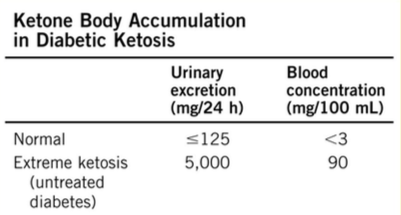
\includegraphics[width=1\textwidth]{fig46}
\caption{Mapa del locus BWS del 11p15.5 \citep{Choufani2010}}
\label{fig46}
\end{figure}

Alteracions epigen�miques i/o gen�miques en el grup de gens \textit{imprinted} en el cromosoma 11p15.5 s'han associat amb BWS en aproximadament el 80\% dels pacients. La regi� 11p15.5 es pot dividir en dos dominis d'\textit{imprinting} diferents separades per una regi� no \textit{imprinted}.

El domini telom�ric/distal 1 cont� els gens \textit{imprinted} IGF2 i H19. Una regi� diferencialment metilat (DMR), 2 kb \textit{upstream} de H19, �s el centre d' \textit{imprinting} putatiu (IC1). El gen H19 expressat maternalment codifica un transcrit de RNAPolII no tradu�t que pot funcionar com un supressor de tumors. El gen IGF2 codifica una citocina expressada paternalment que juga un paper important com un factor de creixement.

Un dels mecanismes de regulaci� �s la regulaci� rec�proca dels gens H19 (expressi� monoal�l�lica materna) i IGF-2 (expressi� monoal�l�lica paterna). IC1 regula l'expressi� \textit{imprinted} d'H19 i IGF2 funcionant com un \textit{insulator}. Al cromosoma matern, IC1 no est� metilat, permetent la uni� de CTCF. Aquesta uni� l'acc�s del promotor IGF2 a \textit{enhancers} que es troben \textit{downstream}. Per tant, la c�pia materna d'H19 utilitza aquests \textit{enhancers} i es transcriu. Al cromosoma patern, la metilaci� de IC1 impedeix la uni� de la prote�na CTCF a IC1, de manera que el promotor IGF2 t� acc�s als \textit{enhancers} i s'expressa mentre H19 �s silenciada.

Els pacients BWS amb alteracions en el domini 1 demostren l'augment de la metilaci� en IC1, �s a dir, la metilaci� es produeix tant en el matern i patern IC1. Aquest canvi en la metilaci� pot oc�rrer com una alteraci� epigen�tica a�llada o en associaci� amb una alteraci� gen�mica subjacent. Les alteracions gen�miques en el domini 1 associades amb BWS s�n microdelecions de longitud variable. La transmissi� materna d'aquesta alteraci� gen�mica s'associa amb BWS, mentre que la transmissi� paterna no ho �s, ja que aquest �ltim al�lel �s normalment metilat. En els casos espor�dics amb un canvi en la metilaci� H19 no associat amb una alteraci� gen�mica subjacent, la marca epigen�tica pot ser normalment reprogramada en la l�nia germinal. Les alteracions epigen�tiques a�llades estan associats amb un baix risc de recurr�ncia, mentre que les delecions gen�miques transmeses per via materna tenen un risc de recurr�ncia del 50\%.

En el domini centrom�ric/proximal 2, el cl�ster \textit{imprinted} abasta una regi� d'1 Mb que cont� aproximadament 10 gens impresos. Dos d'aquests gens, KCNQ1OT1 i CDKN1C, estan clarament implicats en BWS. KCNQ1OT1 �s una transcrit no tradu�t expressat paternalment, llegit en una direcci� antisentit pel que fa al KCNQ1. L'extrem 5 ' de KCNQ1OT1 funciona com el IC2 per al domini 2. En BWS, la p�rdua de metilaci� materna de IC2 est� associat amb l'expressi� de l'al�lel matern normalment silenciat del transcrit KCNQ1OT1. KCNQ1OT1 regula negativament en cis l'expressi� de diversos gens impresos en el domini 2.

El transcrit del KCNQ1OT1 de ratol� exerceix el silenciament espec�fic d'al�lel mitjan�ant l'establiment d'un compartiment nuclear en qu� es troben els gens silenciats. Aquest compartiment de la cromatina s'enriqueix amb marques repressives d'histones (com ara H3K9me3  i/o H3K27me3) i prote�nes Polycomb (com ara EZH2), i �s generalment desprove�t de H3K4me2, una marca d'histona activa que resulta en el silenciament dels gens de tot el domini.

Els defectes d'\textit{imprinting} en IC2 representen la majoria (50\%) dels defectes moleculars en pacients BWS. En la majoria dels casos, aix� es produeix com una alteraci� epigen�tica sense una alteraci� gen�mica subjacent. Per a aquestes fam�lies, el risc de recurr�ncia �s molt baix. Les microduplications/microdelecions que afecten el domini 2 s�n rares.

Altres gens importants en l'etiologia de BWS s�n KCNQ1 i CDKN1C. KCNQ1 �s un transcrit expressat maternalment en la majoria dels teixits amb l'excepci� del cor. El producte del gen KCNQ1 forma part d'un canal de potassi. Aquest gen cont� sis llocs de translocaci� coneguts, tots associats amb qualsevol BWS o tumors. Algunes translocacions o inversions del cromosoma 11p15.5 estan associades amb BWS despr�s de la transmissi� materna de la reordenaci�. La majoria dels pacients amb BWS que tenen una translocaci� o inversi� del cromosoma 11p15.5 no mostren canvis en la metilaci� en IC2.

CDKN1C (p57KIP2) �s un gen expressat maternalment que codifica un inhibidor de la CDK que regula negativament la proliferaci� cel�lular. Les mutacions en CDKN1C es documenten en el 10\% dels pacients amb BWS.

Les alteracions moleculars que afecten els dominis 1 i 2 associades amb BWS:
\begin{itemize}
\item \textbf{Disomia uniparental paterna:} La disomia uniparental paterna involucrant els grups de gens impresos en el cromosoma 11p15 (que abasta IC1 i IC2) es troba en el 20\% dels casos BWS. At�s que tots els casos informats de BWS amb UPD demostren t�picament mosa�cisme som�tic, aquesta alteraci� molecular probable resulta de la recombinaci� som�tica post-zig�tica. �s possible que els embrions amb UPD completa (�s a dir, no mosaic) no s�n viables. Aix� suggereix que l'expressi� del gen impr�s normal en aquesta regi� cromos�mica �s un requisit per al desenvolupament embrionari primerenc.

\item \textbf{Anomalies del cromosoma 11p15 dels dominis 1 i 2:} Rares vegades (1\%) les duplicacions citogen�ticament detectables donen lloc al fenotip BWS. duplicacions patern de 11p15 poden resultar en BWS; duplicacions materns de la mateixa regi� en 11p15 poden resultar en RSS. RSS i BWS fenotips Recentment s'han associat amb duplicacions de 11P en una sola fam�lia.
\end{itemize}

En la gametog�nesi, es borren les marques d'imprinting i es tornen a dipositar.

\subsection{S�ndrome de Prader-Willi i Angelman}
\label{sec:sindrome-de-prader}

Les dues s�ndromes tenen una incid�ncia d'1/15.000 naixements i es caracteritzen per problemes de desenvolupament, comportament i neurol�gics.

\begin{table}[H]
  \centering
  \begin{tabular}{cc}
\hline 
\textbf{S�ndrome d'Angelman} & \textbf{S�ndrome de Prader-Willi}\tabularnewline
\hline 
\hline 
At�xia & Hipotonia neonatal\tabularnewline
Tremolor & Hiperf�gia i obesitat\tabularnewline
Epil�psia & Hipogonadisme\tabularnewline
Problemes per dormir & Estatura baixa\tabularnewline
Hiperactivitat & Mans i peus petits\tabularnewline
Retard mental sever & Retard mental\tabularnewline
Falta de parla & Comportament obsessiu-compulsiu\tabularnewline
Disposici� alegre & \tabularnewline
\hline 
\end{tabular}
  \caption{S�mptomatologia de Prader-Willi i Angelman}
  \label{tab:praderwilli}
\end{table}

El 70\% dels casos es deu a delecions. Tamb� es troben disomies uniparentals, mutacions puntuals (nom�s en Angelman), defectes d'\textit{imprinting} o translocacions balancejades.

Les delecions i casos de disomia unpiparental demostren que a la regi� 15q11-13 hi ha gens \textit{imprinted}. Els gens funcionals s�n els paterns.

\begin{itemize}
\item Si es silencien els gens marcats paterns: S�ndrome de Prader-Willi
\item Si es silencien els gens marcats materns: S�ndrome d'Angelman
\end{itemize}

PWS se sap que �s causada per la falta d'expressi� de gens heretats per via paterna en el cromosoma 15q11-q13, mentre que AS �s causada per la falta d'un �nic gen expressat, UBE3A, a partir del cromosoma 15 d'her�ncia materna. En aquesta regi�, els gens d'her�ncia materna relacionats amb PWS normalment no s'expressen, havent estat torna inactiu a causa de l'empremta gen�tica; Aix� mateix, el UBE3A heretat per via paterna normalment no s'expressa a causa de la impressi� \citep{Cassidy2000}.

\begin{figure}[H]
\centering
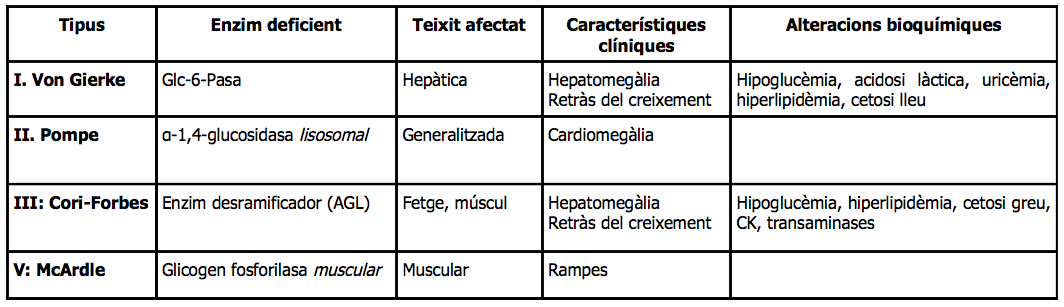
\includegraphics[width=1\textwidth]{fig47}
\caption{Mapa gen�tic de 15q11-13}
\label{fig47}
\end{figure}

\subsubsection{Gen UBE3A}
\label{sec:gen-ube3a}

Se sap que la s�ndrome que �s causada per mutacions o disfunci� en el gen de la ubiquitina ligasa, UBE3A. Mutacions a UBE3A causen el truncament de E6-AP, el que porta a la haploinsufici�ncia de la prote�na. quantitats cel�lulars redu�des de E6-AP semblen no tenir cap efecte en les c�l�lules som�tiques perqu� l'altre al�lel normal al cromosoma 15 patern �s actiu i produeix una quantitat aparentment suficient de prote�na. No obstant aix�, hi ha poca o cap expressi� d'E6-AP del cromosoma 15 patern en certes regions del cervell (c. Purkinje, neurones de l'hipocamp, c. mitrals olfactives), el que reflecteix l'estat de UBE3A Impresa. Per tant, aquestes regions depenen �nicament de la mare UBE3A transcrit.

AS �s causada per diversos mecanismes gen�tics que pertorben l'expressi� UBE3A del cromosoma 15 normal, matern. Els mecanismes conceptualment m�s simples impliquen microdelecions cromos�miques (70\% dels casos), mutacions UBE3A intragenic, i UPD paternal.

E6-AP t� diferents dominis:
\begin{itemize}
\item Domini de co-activaci�
\item Domini d'interacci� amb el receptor de progesterona
\item Domini HECT
\item Domini Ubq-lligasa
\end{itemize}

Els assajos funcionals d'al�lels mutats d'UBE3A mostren que les mutacions assajades eliminen la capacitat d'ubiquitinitzaci� i no afecten la funci� coactivadora. Els car�cters neurol�gics del s�ndrome d'Angelman s�n probablement deguts a un d�ficit en la degradaci� de prote�nes mediada pel proteasoma. E6-AP interacciona amb p53, Src, HHR23A i HHR23B.

Les possibles causes del fenotip neurol�gic de la s�ndrome d'Angelman s�n:
\begin{itemize}
\item  Anomalies en la degradaci� de neurotransmissors
\item Problemes de manteniment o desenvolupament de les sinapsis
\item Degradaci� anormal de prote�nes citoplasm�tiques o nuclears necess�ries per al proc�s de LTP (long term potentiation, en comunicaci� entre neurones)
\item Problemes de regulaci� de prote�nes canal
\item Toxicitat directa de les dianes de E3 no degradades
\item Efectes indirectes de l'acumulaci� de prote�nes inhibidores
\end{itemize}

Hi ha aproximadament 50 mutacions \textit{de novo} o heretades a al�lel matern, el 50\% dels fills de mares portadores seran afectes per� el 0\% dels fills dels pares portadors seran afectes.

\subsubsection{S�ndrome de Prader-Willi}
\label{sec:sindrome-de-prader-1}

No hi ha cap cas de PWS amb mutaci� puntual en un �nic gen. El fenotip PWS, per tant, probablement resulta de la manca d'expressi� del grup de gens contigus marcats de la regi� de 15q11-13 que normalment s'expressen per via paterna.

Els gens marcats amb 15q11-13 amb expressi� exclusiva de l'al�lel matern:
\begin{itemize}
\item ZNF127 = MKRN3
\item MAGEL2: expressi� a l'hipot�lem
\item NDN: necdina, expressi� predominant a neurones post-mit�tiques. Uneix factors de transcripci�.
\item IC/SNURF-SNRPN: locus molt complex
\item PAR-5/IPW/PAR-1: gens que es transcriuen per� no es tradueixen.
\end{itemize}

A m�s, hi ha 3 gens per snoRNA intercalats en introns dels gens anteriors.

El locus SNURF-SNRPN �s un dels candidats ja que cont� els punts de ruptura de 5 pacients PWS amb translocacions balancejades. Cont� tamb� microdelecions en alguns pacients PWS amb mutacions d'\textit{imprinting}. El locus SNURF-SNRPN cont� part del IC (\textit{imprinting center}), codifica la prote�na SmN i SNURF o codifica un dels snoRNA:
\begin{itemize}
\item SmN: exons del 4 al 10 de SNRPN. �s una prote�na del spliceosoma, espec�fica de cervell.
\item SNURF (SNRPN Upstream Reading Frame): �s una prote�na de 71 amino�cids i no est� clara la seva funci�.
\item snoRNA: s�n RNA nucleolars. Estan codificats als introns d'altres gens. Es processen a partir de transcrits primaris i participen en la madduraci� del rRNA.
\item HBII-13, HBII-85 i HBII-52 s�n espec�fics de cervell, marcats amb \textit{imprinting}, expressats nom�s a partir de l'al�lel matern.
\end{itemize}

Necdina i MAGEL2 pertanyen a una gran fam�lia g�nica amb domini MAGE. Tenen patrons d'expressi� compatibles:
\begin{itemize}
\item Necdina: En moltes neurones en estat de post-diferenciaci� (tamb� en m�sucl, pell o cart�lag en desenvolupament).

\item MAGEL2: Neurones de l'hipot�lem en vies de desenvolupament. 
\end{itemize}

Els experiments d'expressi� in vitro mostren que la necdina t� un paper en la diferenciaci� neuronal
terminal. Els experiments de two-hybrid demostren que la necdina i Magel2 interactuen amb prote�nes
implicades en la reorganitzaci� del citoesquelet intervinguda pel centrosoma, creixement d'axons i neurites, i finalment diferenciaci� neuronal.

Els defectes d'\textit{imprinting} que causen PWS o AS expliquen el 5\% de cada patologia. Un 50\% tenen delecions submicrosc�piques que afecten el centre d'\textit{imprinting}. El 50\% no tenen deleci� ni mutaci�, amb un marcatge an�mal o epigenotip. 

Les microdelecions dels pacients PWS i AS defineixen les regions PWS SRO i AS SRO. Les SRO s�n les \textit{Shortest Region of Overlap}. Les SRO han de tenir seq��ncies implicades en determinar l'\textit{imprinting}.

\begin{figure}[H]
\centering
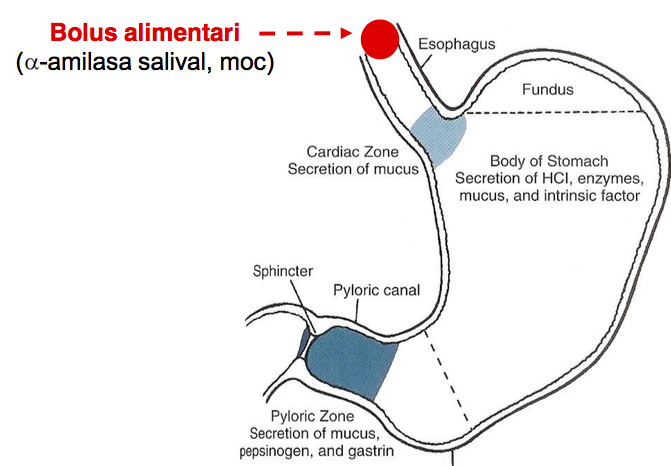
\includegraphics[width=0.8\textwidth]{fig48}
\label{fig48}
\end{figure}

Aquesta regi� AS-SRO de 2 kb est� dins el intr� 3 d'una transcrit nou en l'IC, representant exons alternatius a 5' del gen SNRPN. Aquests 5 exons s'expressen aproximadament 100 vegades menys en les c�l�lules som�tiques que el transcrit SNRPN que s'inicia en una illa CpG. Els exons 5' es denominen ara com a transcrit IC, ja que est� postulat per tenir una funci� diferent a la de la funci� de codificaci� de prote�na de SNRPN. Igual que SNRPN, el transcrit IC s'imprimeix i nomes s'expressa paternalment en el cervell i el cor. En PWS, un SRO de 4 kb es defineix per an�lisi de set microdelecions. Aquesta regi� defineix l'element cr�tic que canvia l'\textit{imprinting} patern-matern en la l�nia germinal masculina. El PWS-SRO inclou l'ex� 1 i el promotor d'una illa CpG del gen SNRPN \citep{Saitoh1998}.

SNRPN cont� dues regions amb \textit{imprinting}: la regi� del ex� 1, que �s l'al�lel patern no metilat i expressat i l'al�lel matern metilat silenciat; i una regi� en l'intr� 7, que est� metilat al patern i no al matern \citep{Saitoh1998}.

Les microdelecions associades amb la s�ndrome d'Angelman (AS) s�n en general a la regi� \textit{upstream} de SNRPN i estan associades amb la p�rdua de la metilaci� en la regi� promotora de SNRPN materna, i probablement tamb� amb els canvis en la metilaci� i l'expressi� del gen UBE3A expressat maternalment. La p�rdua de la funci� d'UBE3A sembla ser responsable de moltes de les caracter�stiques de la AS. Sorprenentment, les supressions relacionades amb AS no necess�riament inclouen el gen UBE3A, per� freq�entment afecten exons d'un transcript alternatiu de SNRPN que cont� diversos exons localitzats a la regi� \textit{upstream} d'aquest gen. S'ha suposat que aquesta regi� cont� un IC que �s necessari per a la regulaci� dels gens expressats per via materna. El mecanisme d'impressi� relacionat podria estar mediat per la transcripci� activa de transcrits alternatius de SNRPN. Recentment, la zona s'ha redu�t a 880 pb. Aquesta superposici� es creu que representen el IC d'AS que �s necessari per a la impressi� correcta de l'al�lel matern \citep{Paulsen2001}.

Un efecte de llarg abast es podria aconseguir mitjan�ant la interacci� de diversos elements que es dispersen per tota la regi�. La regi� promotora de SNRPN �s important no nom�s per l'interruptor de la l�nia germinal de la mare a l'empremta paterna, sin� tamb� per al canvi de la marca de l'empremta paterna. La regi� promotora de SNRPN regula la impressi� no nom�s de SNRPN, sin� tamb� de tota la regi�. Els pacients que tenen translocacions amb punts d'interrupci� telom�rica de SNRPN exhibeixen impressi� adequada de SNRPN per� no de gens distals dels punts d'interrupci� de translocaci�.

Els IC de PWS i AS de fet exhibeixen estructures de la cromatina espec�fiques d'al�lel. La cromatina del IC de PWS semblava ser hipersensible a la nucleasa en l'al�lel patern i es troba al costat dels llocs en el primer intr� SNRPN que s�n sensibles a la nucleasa a l'al�lel matern. Aix� suposaria una major accessibilitat del IC de PWS a les prote�nes d'uni� al DNA en l'al�lel patern, permetent d'aquesta manera les interaccions en cis amb regions flanquejants necess�ries per al manteniment de l'empremta paterna en aquesta regi�. La situaci� oposada a l'intr� 1, hipersensibilitat a la nucleasa en  l'al�lel matern per� menys sensibilitat per l'al�lel patern, podria indicar una difer�ncia funcional intervinguda per l'estructura de la cromatina. La creaci� o el manteniment de l'empremta materna s'activa per la uni� de factors proteics a aquesta regi� \citep{Paulsen2001}.

UBE3A-AS �s d'expressi� excluivament paterna i espec�fica del cervell. Expressa un transcrit antisentit que bloqueja l'expressi� de l'al�lel patern de UBE3A.

%------------------------------------------------------------------------------
% Tema 11. Aparell digestiu
%------------------------------------------------------------------------------
\newpage
%%------------------------------------------------------------------------------
% Tema 11. Cerca d'un gen per exoma. Opitz C
%------------------------------------------------------------------------------
\section{Cerca d'un gen per exoma. Opitz C}
\label{sec:cerca-dun-gen}

Un anàlisi per WES d'una pacient va donar una mutació en heterozigosi p.Q638 a MAGEL2. La mutació es manifestava com a dominant.

Es van publicar diverses mutacions a MAGEL2 amb fenotip similar a Prader-Willi però no com a Opitz C.

MAGEL2 es troba a la regió associada amb Prader-Willi, i té expressió paterna (l'al·lel matern està silenciat).

Per determinar la fase: van digerir el genoma amb un enzim sensible a metilació.

En alguns casos, el pare té la mutació però heratat de la mare; llavors no té cap fenotip.

MAGEL2 s'uneix i activa a E3 RING Ubq lligases. Implicat en SUMOilació i transport retrògrad (de l'endosoma a Golgi).

També s'han trobat mutacions a TRAF7 (transducció de senyal, E3 Ubq lligasa).

Una altra mutació en FOXP1, una mutació \textit{de novo} wt/c.1428+1G>A a una regió donadora d'splicing.

%------------------------------------------------------------------------------
% Tema 12. Alteracions del metabolisme de nucle�tids
%------------------------------------------------------------------------------
\newpage
%%------------------------------------------------------------------------------
% Tema 12. Defectes del tancament del tub neural
%------------------------------------------------------------------------------
\section{Defectes del tancament del tub neural}
\label{sec:defect-del-tanc}

\subsection{El tub neural}
\label{sec:el-tub-neural}

Els defectes del tub neural s�n obertures de la medul�la espinal o del
cervell que tenen lloc en etapes molt primerenques del
desenvolupament. En aquest estadi, la placa neural es plega i forma el
tub neural. Aquest tub neural despr�s donar� lloc al cervell i la
medul�la espinal. Els NTDs s�n errors en el proc�s de tancament del
tub neural.

En primer lloc, es forma la placa neural. Despr�s t� lloc una elevaci�
de les parets neurals per formar el solc neural. Despr�s les parets
convergeixen per formar els plegaments neurals i finalment es fusionen
per tancar el tub.

\begin{figure}[H]
\centering
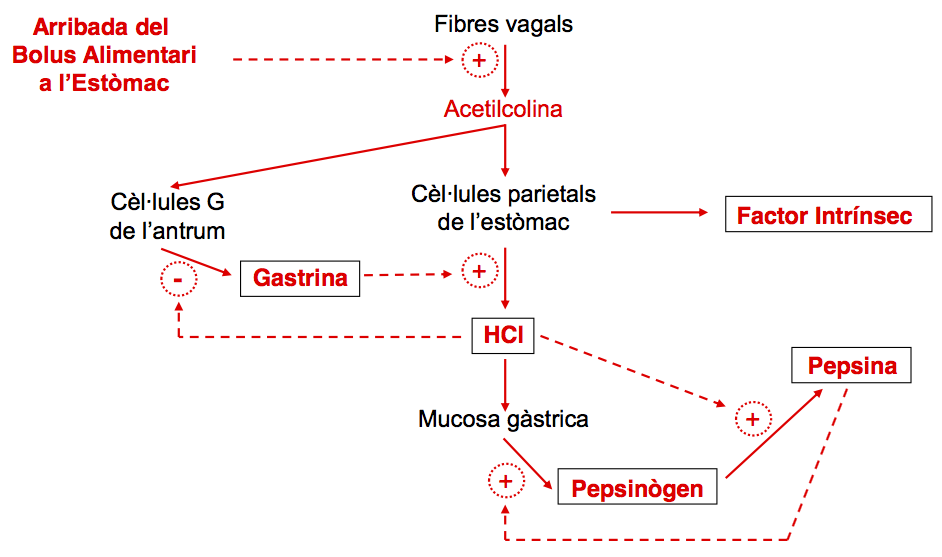
\includegraphics[width=1\textwidth]{fig49}
\label{fig49}
\end{figure}

\subsection{Defectes del tub neural}
\label{sec:defectes-del-tub}

A l'hum� els m�s freq�ents s�n:
\begin{itemize}
\item \textbf{Anencef�lia:} Manca de cervell frontal, meninges corresponents,
  crani corresponent i pell corresponent. Incompatible amb la vida.

\item \textbf{Espina b�fida:} Arcs vertebrals lumbars sense
  soldar. L'espina b�fida \textit{occulta} nom�s afecta l'os i
  l'espina b�fida \textit{apperta} inclou la protrusi� de les meninges
  (meningocele) o de meninges i elements neurals
  (meningomielocele). T� diferents problemes associats, com la
  hidrocef�lia (increment l�quid cefaloraquidi al cervell), par�lisi
  de les cames i risc d'infecci� si l'obertura no est� coberta per
  pell; sempre s'ha d'operar per tancar la medul�la, per� poden quedar
  seq�eles.
\end{itemize}

\begin{table}[H]
  \centering
  \begin{tabular}{|c|c|}
\hline
\hline 
Promig mundial & 1/500\tabularnewline
USA & 1/3300\tabularnewline
Finl�ndia & 1/2500\tabularnewline
Holanda & 1/700\tabularnewline
M�xic & 1/300\tabularnewline
Gales & 1/80\tabularnewline
Irlanda & 1/100\tabularnewline
\hline 
\hline
\end{tabular}
  \caption{Indic�ncia poblacional de NTD}
  \label{tab:ntd}
\end{table}

Tenen una gran variaci� �tnica i geogr�fica degut a difer�ncies de
susceptibilitat gen�tica, culturals, nutricionals.

L'etiologia dels NTD �s clarament multifactorial:
\begin{itemize}
\item Factors intr�nsecs / extr�nsecs
\item Factors gen�tics / ambientals
\item Alguns pocs factors identificats
\item Relaci� entre factors gen�tics i ambientals desconeguda
\end{itemize}

Els NTDs s�n exemple de malaltia gen�tica COMPLEXA.

\subsection{Car�cters multifactorials}
\label{sec:caract-mult}

Un car�cter multifactorial �s aquell a causa d'una combinaci� de
diversos factors gen�tics i no gen�tics, on cada un d'ells juga un
paper relativament petit.

Alguns exemples s�n:
\begin{itemize}
\item Malformacions cong�nites
  \begin{itemize}
  \item Llavi lepor� (0.4-1.7/1000)
  \item Paladar fes (0.4/1000)
  \item Luxaci� cong�nita del maluc (2/1000 en homes)
  \item Cardiopaties cong�nites (4-8/1000)
  \item Defectes del tub neural (2-10/1000)
  \item Estenosi pil�rica (1 en dones i 5/1000 en homes)
  \end{itemize}
\item Patologies comunes de l'adult
  \begin{itemize}
  \item Diabetis mellitus
  \item Malalties cardiovasculars
  \item Osteoporosi
  \item Esquizofr�nia
  \end{itemize}
\end{itemize}

A inicis del 1900 Francis Galton va observar que els car�cters m�s
importants dels humans s�n car�cters que no es poden calcular com
unitats discretes, �s a dir, que no es definien per car�cters
mendelians.

Al 1918 R.A. Fisher va proposar el model polig�nic, que deia que
unitats discretes mendelians es poden expressar com car�cters
complexos si aquests existeixen de manera independent en diferents
gens. Aquests car�cters polig�nics mostren una variaci� cont�nua i
correlacions familiars. Anys m�s tard Falconer va fer el model
llindar, que explica els trets dicot�mics que no explicava el model de
Fisher.

\subsubsection{Model polig�nic d'her�ncia de car�cters quantitatius}
\label{sec:model-polig-dher}

Explica que els trets complexos depenen del efecte additiu de
m�ltiples factors individuals petits i additius i que tenen una
distribuci� normal a la poblaci�.

S�n loci on cada al�lel dominant afegeix unitats additives; quan hi ha
un major nombre de loci implicats hi ha tamb� un augment de les
classes fenot�piques.

Els car�cters que s'expliquen amb aquest model presenten el fenomen de
regressi� a la mitja, que consisteix en qu� el fenotip de descendents
d'encreuaments d'individus dels extrems �s un fenotip intermedi dels
gens dels pares i la mitjana de la poblaci�. Aquest fenomen �s
purament estad�stic, i dep�n de les propietats de la corba de la
distribuci� normal, que mant� la variabilitat.

Aquest model es basa en que sempre es produeix panmixia i que no hi ha
una domin�ncia. Suposem que no hi ha domin�ncia, i que es tracta d'un
proc�s atzar�s. Pot donar lloc a males interpretacions, com per
exemple dir que despr�s de poques generacions tots seran iguals, o dir
que es tracta d'un mecanisme gen�tic, quan ja hem dit que �s un
fenomen purament estad�stic.

Les malalties mendelianes tenen al�lels mutants rars, amb penetr�ncia
alta. Degudes a mutacions.

Les malalties complexes tenen al�lels mutants freq�ents amb una
penetr�ncia baixa. Degudes a polimorfismes.

Les malformacions cong�nites i moltes de les patologies comunes de
l'adult s�n multifactorials per� NO s�n car�cters quantitatius.

\subsubsection{Model del llindar}
\label{sec:model-del-llindar}

Com ja hem comentat, aquest model �s una extensi� del model polig�nic
de Fisher que avarca tamb� els car�cters dicot�mics.

Es defensa que totes les persones d'una poblaci� tenen uns determinats
factors de risc, uns valors de susceptibilitat que, en sobrepassar un
llindar, provoquen l'expressi� d'un fenotip determinat.

La susceptibilitat �s el conjunt dels valors o factors de risc que, en
sobrepassar aquest llindar, causen un fenotip concret. Aquest fenomen
explica el risc de recurr�ncia en fam�lies.

Quan existeix una difer�ncia sexual en el llindar, �s a dir, que el
llindar �s diferent en homes i en dones, ens trobem en una situaci� en
que els individus de diferents sexes presenten diferents factors de
susceptibilitat. A vegades existeix tamb� una difer�ncia de llindars
entre diferents individus, independentment del sexe.

Aquest model tamb� explica les difer�ncies de risc i de
susceptibilitat entre les fam�lies, ja que compartim tant els gens com
l'ambient.

En resum, com m�s gran �s el llindar m�s gran �s el nombre de gens que
controlen la malaltia. 

Una manera de comprovar que el car�cter complex estudiat t� una
variant gen�tica �s a trav�s de l'agregaci� familiar, ja que si
realment es tracten de car�cters amb una base gen�tica observarem
fen�mens d'agregaci� familiar, ja que aquests trets presenten una
recurr�ncia en fam�lies.

En malalties mendelianes el risc variar� de manera gradual en funci�
del grau de parentesc, mentre que a les malalties complexes observarem
una variaci� cont�nua m�s sobtada i imprevisible.

En aquests estudis es calcula la r�tio de risc de recurr�ncia
familiar, FRR, \textgreek{l}R, �s a dir, el risc de patir la malaltia
tenir un familiar afectat respecte el risc normal de patir la malaltia
en la poblaci� general. �s una mesura d'agregaci� familiar.

Es calcula el risc de recurr�ncia a partir de freq��ncies familiars
poblacional. Quan la r�tio de risc de recurr�ncia, �s a dir, la FRR,
�s major a 1, aix� �s indicatiu que existeix una situaci� d'agregaci�
familiar i que hi ha una base gen�tica en el car�cter estudiat.

Nom�s podem afirmar que hi ha base gen�tica quan \textgreek{l}>10. La
FFR tamb� �s �til per deduir efectes additius o multiplicatius en
aquest tipus de car�cter, aix� com per crear models gen�tics que
puguin explicar aquestes malalties complexes.

El risc de recurr�ncia disminueix en allunyar el parentesc, i ho fa de
manera irregular.

\subsection{NTD gen�tic}
\label{sec:factors-genetics-de}

El fet que hi hagi recurr�ncia en fam�lies suggereix que en la
patologia hi ha una base gen�tica. Per� NO �s una prova
definitiva. Les fam�lies, a m�s de compartir gens, tamb� comparteixen
un ambient i estil de vida.

\subsubsection{Estudis de bessons}
\label{sec:estudis-de-bessons}

Aquest tipus d'estudi es basen en comparar el grau de similitud entre
parelles de bessons monozig�tics (MZ) i dizig�tics (DZ). A partir de
les concordances entre els bessons es calcula si �s un car�cter
quantitatiu. Cal tenir en compte que els bessons monozig�tics
comparteixen el 100\% del genoma, mentre que els dizig�tics nom�s un
50\%.

Aleshores, si es tracta d'un car�cter discontinu hi haur� concordan�a
entre els bessons, mentre que si parlem de car�cters continus, com ara
l'estatura, hi haur� una correlaci� o regressi� entre els bessons, no
una concordan�a exacta.

Aquest estudi ens permet calcular tamb� l'heretabilitat del car�cter,
�s a dir, mesurar la proporci� d'her�ncia que �s deguda a factors
gen�tics.

L'heretabilitat d'un car�cter totalment gen�tic ser� de 1; hi ha
concordan�a del 100\% en monozig�tics i concordan�a del 50\% en
dizig�tics. En aquest cas, com que el car�cter �s totalment gen�tic,
l'ambient no afecta per res.
\begin{equation}
h^2 = 2 C_{MZ} - C_{DZ} = 2 r_{MZ} - r_{DZ}
\end{equation}

On C\textsubscript{MZ} �s la correlaci� dels monozig�tics,
C\textsubscript{DZ} la correlaci� dels dizig�tics, i
r\textsubscript{MZ} i r\textsubscript{DZ} les respectives regressions.

Hi ha molts pocs casos de bessons amb NTD, pel que �s pr�cticament
impossible comparar MZ amb DZ.

\subsubsection{Associaci� de NTDs amb algunes s�ndromes monog�nics}
\label{sec:associacio-de-ntds}

Hi ha 2 s�ndromes principals:
\begin{itemize}
\item S�ndrome de Meckel-Gruber (AR): molts tipus de malformacions,
  entre elles, encefalocele.

\item S�ndrome de Waardenburg (AD): problemes de pigmentaci� i
  sordesa; de vegades espina b�fida. Gen PAX3.
\end{itemize}

\subsubsection{Cromosomopaties}
\label{sec:cromosomopaties}

En conjunt, es troben en el 5-17\% dels NTD prenatals. Les m�s
recurrents s�n les trisomies 13 i 18.

\subsection{Factors ambientals de risc per NTD}
\label{sec:fact-ambi-de}

En trobem de 2 tipus:
\begin{itemize}
\item Preventius: �cid f�lic

\item Agents teratog�nics que causen o confereixen un risc superior de
  patir malformacions cong�nites.
\item F�rmacs anticonvulsius contra l'epil�psia
  \begin{itemize}
  \item �cid valproic (RR=1-2\%)
  \item Carbamacepina (RR=0,5\%)
  \end{itemize}
\item Diabetis
\item Obesitat (BMI > 29)
\item Hipert�rmia
\end{itemize}

El 1964 Hibbard va conduir un estudi retrospectiu amb dones amb fills
amb NTDs, i presentaven incid�ncia m�s alta d'errors en el metabolisme
del folat. En 1976 Smithells i cols van fer un estudi durant l'embar�s
i obtenien una mesura del folat del primer trimestre i van trobar que
les dones amb fills amb NTDs tenen nivells de folat eritrocitari
inferiors a mares de fills sense NTDs.

La hip�tesi �s que la ingesta de folat en el temps de la concepci�
podria protegir contra l'aparici� de NTDs. Les concepcions al final de
l'hivern (menys disponibilitat de vegetals) tenen risc m�s elevat de
NTDs. Les concepcions en entorns socioecon�mics pobres tamb� tenen
risc incrementat de NTDs. En �poques de guerra (disponibilitat molt
limitada d'aliments en general i vitamines en particular) s'han
reportat incid�ncies m�s altes de NTDs.

Els estudis de prevenci� de recurr�ncia de NTD es basaven en el
subministrament d'�cid f�lic en el temps de la concepci� a
embarassades que ja tenien un fill amb NTD. El folat, per si sol, va
reduir la recurr�ncia de NTDs en un 72\%. El suplement multivitam�nic
sol, o els minerals van ser inefectius.

Com que el 5\% dels casos s�n recurrents en fam�lies i el 95\% s�n
casos \textit{de novo}, la q�esti� era si aquests �ltims casos tamb�
es podien prevenir amb folat. Els estudis de prevenci� d'incid�ncia de
NTDs es basaven en el subministrament d'�cid f�lic en el temps de la
concepci� a embarassades que no tenien un fill amb NTD. L'estudi de
Budapest de  Czeizel i Dubtes en 1992 comprenia m�s de 4000 dones amb
plans d'embar�s i els resultats van replicar.

Actualment, s'accepta que el suplement de folat en el temps de la
concepci� redueix tant la recurr�ncia com la incid�ncia de
NTDs. Diversos governs recomanen a les dones amb plans d'embar�s que
prenguin dosis de folat de 0,4-0,5 mg / dia per a prevenir els NTDs i
4-5 mg / dia per a prevenir la recurr�ncia de NTDs. En USA, des de
1993, el govern va decidir fortificar els cereals i la farina amb �cid
f�lic (1,4 mg / kg) perqu� la poblaci� en general prengui m�s folat.

\subsection{Factors gen�tics pels NTD relacionats amb el folat}
\label{sec:fact-genet-pels}

\subsubsection{Metabolisme del folat i enzims implicats}
\label{sec:metab-del-folat}

En mam�fers, el folat �s substrat de diversos cicles metab�lics:
\begin{itemize}
\item Bios�ntesi de timidilats i purines
\item S�ntesi de metionina per remetilaci� d'homociste�na
\item Interconversi� de serina i glicina
\item Metabolisme de la histidina i del format
\end{itemize}

Hi ha una llista llarga d'enzims (i gens) candidats com a factors de
susceptibilitat pels NTDs.

\subsubsection{Folat i homociste�na}
\label{sec:folat-i-homocisteina}

L' homociste�na �s un amino�cid absent en la dieta. Es forma per
desmetilaci� de la metionina. Pot remetilar-se a metionina obtenint el
grup metil del 5-MeTHF. �s t�xica per a l'organisme. La homocistin�ria
�s una patologia monog�nica amb elevat risc d'accident vascular
prematur. La hiperhomocistein�mia presenta risc d'accidents vasculars.

En 1991 Steegers-Theunissen et al. van veure que les dones amb fills
amb NTDs tenen nivells plasm�tics de Hcy m�s alts que en controls. Les
variants dels gens relacionats amb Hcy podrien ser responsables de la
hiperhomocisteinemia (i aquesta ser en part responsable dels
NTDs). Les pacients podrien respondre a dosis suplement�ries de folat.

Els nivells de tHcy depenen, entre d'altres, dels gens que codifiquen
pels enzims CBS (cistatlonina $\beta$ sintetasa), MTHFR (metilen THF
reductasa) i MS (metionina sintetasa).

Al gen MTHFR s'han descrit polimorfismes que produeixen un enzim
termosensible, i que s'associen a nivells de folat plasm�tic
disminu�ts i nivells de Hcy plasm�tica augmentats. Els polimorfismes
s�n 677 C>T (Ala>Val) i 1298 A>C (Glu>Ala).

El 1995 - van der Put et al. van trobar que el canvi 677 C> T �s m�s
freq�ent en mares de nens amb NTD i en els propis nens afectes que en
poblaci� control. El canvi 677 C> T confereix un risc de NTDs d'entre
2,9- 3,7 x risc poblacional. El 677C>T �s el primer factor gen�tic per
NTD que s'ha identificat.

%------------------------------------------------------------------------------
% Tema 13. Funci� tiro�dal
%------------------------------------------------------------------------------
\newpage
%%------------------------------------------------------------------------------
% Tema 13. Barreres cel·lulars
%------------------------------------------------------------------------------
\section{Barreres cel·lulars}
\label{sec:barreres-cel.lulars}

\subsection{Entrega sistèmica i barreres extracel·lulars}
\label{sec:entrega-sistemica-i}
Cal tenir en compte que l'entrega sistèmica de material genètic nu, o en vectors virals o físics presenta diferents barreres:
\begin{itemize}
\item \textbf{Metabolisme sistèmic}
  \begin{itemize}
  \item Endonucleases sèriques
  \item Interaccions inespecífiques amb proteïnes
  \item Interaccions específiques amb cèl·lules
  \item Fagocitosi
  \item Excreció renal
  \end{itemize}
\item \textbf{Barreres extracel·lulars:}
  \begin{itemize}
  \item Endoteli
  \item Membranes
  \item Mucus
  \end{itemize}
\item \textbf{Barreres cel·lulars:}
  \begin{itemize}
  \item Interacció amb la superfície cel·lular
  \item Mecanismes d'internalització
  \item Alliberament de les vesícules endocítiques
  \item Mobilitat i estabilitat dels àcids nucleics lliures al citoplasma
  \item Transport al nucli
  \end{itemize}
\end{itemize}

\subsubsection{Metabolisme sistèmic}
\label{sec:metabolisme-sistemic}

\paragraph{Endonucleases sèriques}
Les nucleases del plasma degraden el DNA nu i els oligonucleòtids.
El DNA plasmídic (nu o complexat) administrat per via intravenosa ràpidament es desenrotlla a formes circulars obertes, que estan exposades a les nucleases.

Els siRNAs (o similars) no modificats o sense protecció són degradats per ribonucleases de plasma.

\paragraph{Agregació amb proteïnes sèriques}
Els poliplexes o lipoplexes carregats positivament s'uneixen a les proteïnes del sèrum carregades negativament (com ara albúmina), reduint d'aquesta manera l'eficàcia de la transfecció.
La PEGilació (unió de molècules de polietilenglicol a la superfície de lipoplexes o polipolexes carregats positivament) pot apantallar les càrregues positives i evitar la interacció amb les proteïnes plasmàtiques.

Si la transfecció fos in vitro, no faria falta ja que interessa que el lipoplexe tingui càrrega positiva perquè així interacciona més fàcilment amb la cèl·lula.

La pegilació, és a dir la conjugació amb polietilenglicol (PEG), dels polímers catiònics permet una reducció de la unió no específica a les superfícies cel·lulars.

La pegilació es pot fer reversible via utilització de connectors que es poden trencar per diferents mecanismes.

\paragraph{Agregació amb cèl·lules sanguínies i fagocitosi}
Alguns vectors tipus molècules catiòniques poden unir-se a qualsevol tipus de cèl·lula in vivo incloent cèl·lules de la sang i macròfags.

La unió a cèl·lules sanguínies (riques en heparan sulfats) poden provocar la seva agregació i la formació de trombes.

La unió a macròfags resulta en un aclariment ràpid del torrent sanguini per fagocitosi.

Per exemple: liposomes catiònics convencionals s'eliminen en última instància, de la circulació sanguínia pel sistema dels macròfags.

La PEGilació dels vectors redueix el risc en l'administració intravascular de vectors carregats positivament

\paragraph{Excreció renal}
Molècules de vector neutres, feblement aniòniques o amb càrregues no exposades (vectors PEGilats) tenen poca afinitat per la superfície cel·lular i s'eliminen més lentament, en funció de la seva grandària molecular que determina el seu grau de filtració glomerular renal.

La filtració renal al glomèrul depèn de la mida molecular, les molècules <50 kDa són filtrades, poden ser reabsorbides en els túbuls renals i s'excreten en l'orina.

En conseqüència, les molècules petites per sota del llindar de la mida filtrada al glomèrul s'eliminen ràpidament del plasma per excreció renal.

Els oligonucleòtids i els siRNAs són excretats ràpidament en l'orina; quan es lliguen a vectors s'impedeix l'excreció renal i això és essencial per millorar la farmacocinètica després de l'administració sistemàtica.

\subsubsection{Barreres extracel·lulars}
\label{sec:barr-extr}

\paragraph{Endoteli}
Les grans molècules que circulen en sang només poden accedir a cèl·lules sanguínies, cèl·lules endotelials; i les cèl·lules del parènquima en el fetge i la melsa, que tenen un endoteli discontinu.

En el cas dels capil·lars continus no fenestrats, l'aigua i els soluts petits (radi molecular < 3 nm) passen entre les cèl·lules de l'endoteli, mentre que els soluts més grans passar a través de les cèl·lules de l'endoteli o bé a través de canals transendotelials o transcitosis, intervinguda principalment per cavèoles.

Els capilars continus fenestrats presenten una major permeabilitat a l'aigua i soluts petits, però els coeficients de reflexió similars a macromolècules grans (els diafragmes de la Llei de fenestras com filtres moleculars).

Els capil·lars discontinus i sinusoïdals tenen fenestracions (sense diafragmes), gaps, i una membrana basal mal organitzada. Aquestes cèl·lules endotelials contenen moltes depressions revestides de clatrina, les quals juguen un paper important en l'endocitosi mediada per receptor (encara que també poden prendre part en la transcitosis) que inclou compartiments endosomal i lisosomals.

\paragraph{Membranes}
Estructures de la matriu extracel·lular que separen les cèl·lules del teixit connectiu circumdant. Això es produeix en diversos teixits i tumors sòlids. Les membranes limiten la difusió de les molècules en el teixit.

\paragraph{Mucus}
Secreció viscosa que conté proteïnes que impedeix la difusió de molècules.

\subsection{Interacció cel·lular}
\label{sec:interaccio-cel.lular}
La interacció dependrà de si el vector té:
\begin{itemize}
\item Cobertura amb lligand: Adsorció/adhesió per interacció electrostàtica.
\item Cobertura amb lligand: Reconeixement per una proteïna cel·lular de proteïnes de la càpside viral, altres proteïnes, pèptids RGD o residus glucídics.
\end{itemize}

En el cas dels àcids nucleics nus, el mecanisme és força desconegut.

\subsubsection{Cobertura sense lligand}
\label{sec:cobert-sense-llig}
El vector és adsorbit en la membrana cel·lular depenent de les propietats de bioadhesió. L'abundància de llocs aniònics a la membrana cel·lular (proteoglicans de la superfície cel·lular sulfatats carregats negativament) implica que grups catiònics tenen una tendència a "enganxar-se".

Això ha estat aprofitat en els liposomes catiònics i polímers catiònics.

La PEGilació dels polímers catiònics permet una reducció de la unió no específica a les superfícies cel·lulars.

\subsubsection{Cobertura amb lligand}
\label{sec:cobert-amb-llig}
Les proteïnes lligands són proteïnes que interaccionen amb receptors o antígens de la membrana, lligands o anticossos, respectivament.

Moltes integrines de la superfície cel·lular s'uneixen a les seqüències de pèptids Arg-Gly-Asp (RGD) presents en les proteïnes de matriu extracel·lular i sèrum.

RGD s'utilitza per dirigir la interacció dels vectors amb la cèl·lula mitjançant les integrines. Algunes integrines intervenen a més en la internalització dels lligands RGD a través de la via d'endocitosi. S'usa molt per transfectar tumors.

La mannosa interacciona amb el receptor de mannosa. Aquest s'expressa preferentment a macròfags i cèl·lules dendrítiques. El receptor de mannosa uneix glicoproteïnes que contenen mannosa, glucosa, fucosa i N-acetilglucosamina.

Galactosa: els residus de galactosa acoblats a la polietilenimina (PEI) transfecten de forma selectiva hepatòcits a través del receptor de les asialoglicoproteïnes. Aquest receptor s'uneix naturalment a les asialoglicoproteïnes, això és, glicoproteïnes de les quals ha estat retirat l'àcid siàlic quedant exposats els residus de galactosa.

El receptor de les asialoglicoproteïnes s'expressa a les cèl·lules del fetge per eliminar glicoproteïnes diana de la circulació.

% Taula de lligands de càpsides virals


\subsection{Captació}
\label{sec:captacio}

\subsubsection{Fusió amb la membrana}
\label{sec:fusio-amb-la}
Les cobertures amb determinats lípids fusionen amb la membrana plasmàtica i d'aquesta manera les molècules associades són alliberades directament al citosol.

Els vectors que es fusionen amb la membrana són:
\begin{itemize}
\item Virus amb embolcall lipídic: retrocirus, herpes, vaccinia virus (cowpox).
\item Liposomes
\end{itemize}

\subsubsection{Endocitosi}
\label{sec:endocitosi}
La ruta endocítica per la qual una molècula o virus entra a la cèl·lula és altament dependent de la seva mida, la càrrega i la composició, així com en el tipus de cèl·lula en què està entrant.

\paragraph{Endocitosi mitjançada per receptor}
Procés pel qual les cèl·lules internalitzen molècules en vesícules que contenen les molècules de lligand, en aquest cas molècules del vector (proteïnes, carbohidrats, ..), i el receptor de membrana que reconeix el lligand.

\begin{itemize}
\item \textbf{Vesícules recobertes de clatrina:} la via endocítica implica la fusió d'endosomes amb els lisosomes (vesícules que contenen enzims per la degradació) i per tant la degradació dels vectors i DNA. La mida òptima del lligand és de 100 nm. És utilitzada per adenovirus 2/5, AAV, retrovirus, liposomes i polications petits.

\item \textbf{Caveoles:} la mida típica del lligand és de 500 nm. És utilitzada per polications grans. La captació de molècules també és mitjançada per receptors.

\item \textbf{Lípid rafts:} són microdominis de la membrana cel·lular enriquida en colesterol i esfingolípids. És utilitzada per retrovirus. Les vesícules no dependents de clatrina semblen no fusionar amb els lisosomes i dirigir-se directament al reticle endoplasmàtic.
\end{itemize}

\paragraph{Fagocitosi}
Els fagosomes són vesícules que encapsulen molècules grans. La fagocitosi es realitza principalment per cèl·lules especialitzades en eliminar els patògens de grans dimensions o restes: macròfags i neutròfils. La fagocitosi requereix d'una certa especificitat: la unió del lligand a receptors cel·lulars d'adherència . Els fagosomes maduren per fusionar amb els lisosomes.

\paragraph{Macropinocitosi}
Consisteix en la invaginació de la membrana plasmàtica i formació d'endosomes per captar proteïnes individuals i fluids.

La destinació intracel·lular dels macropinosomes depèn del tipus cel·lular: en els macròfags es fusionen posteriorment amb els lisosomes, mentre que altres cèl·lules, eventualment reciclen la major part dels continguts de tornada a la superfície cel·lular.

Els macropinosomes són inherentment vesícules que degoten en comparació amb altres tipus d'endosomes.

Sembla ser que aquest procés és molt important pels tumors per captar nutrients de l'exterior cel·lular.

\subsubsection{Pèptids de penetració cel·lular}
\label{sec:pept-de-penetr}
Els pèptids de penetració cel·lular (CPPs) presenten diferents mecanismes de translocació de la membrana cel·lular

Alguns CPPs i les seves càrregues poden penetrar directament a través de la membrana plasmàtica, segons els models: 
\begin{itemize}
\item Catifa, en el qual hi ha una desestabilització transitòria de la membrana cel·lular induïda per l'associació del pèptid i reorganització consegüent de fosfolípids.
\item Micel·la invertida, per la pertorbació de la membrana plasmàtica formant una estructura hexagonal en un procés reversible.
\item Porus transitoris produïts després de la inserció i oligomerització dels pèptids en una estructura d'anell de formes diferents.
\end{itemize}

No obstant, en general s'accepta que els CPPs usen sobretot les vies endocítiques per entrar en les cèl·lules. El mètode de captació endocítica varia segons la grandària i la naturalesa del complex COP-àcid nucleic. Poden ser vies dependents de clatrina, vies clatrina-independents i macropinocitosi.

\subsection{Sortida de l'endosoma i estabilitat al citoplasma}
\label{sec:sortida-de-lendosoma}

Estructures hexagonals de fusió: els liposomes catiònics multilaminars després de l'endocitosi formen estructures hexagonals que fusionen amb les membranes aniòniques endosòmiques per alliberar l'àcid nucleic al citosol. Els poliplexos dendrímers també semblen formar aquestes estructures.

Els polications tipus poliamines actuen com una esponja que atrapa H+, Cl- i aigua, infla els endosomes i fa que esclatin alliberant el seu contingut al citosol.

També tenen un efecte paraigües: la protonació de les amines al baix pH fa que el polímer passi d'una conformació condensada a un estesa.

Alguns àcids nucleics són efectius al citosol.
\begin{itemize}
\item mRNAs sintètics (modificades químicament) codificants de proteïna.
\item Oligonucleòtids antisentit.
\item siRNAs.
\item miRNAs.
\end{itemize}

El DNA codificant ha d'arribar al nucli per ser transcrit. Entre aquests:
\begin{itemize}
\item DNA codificant per proteïna.
\item DNA codificant per RNA antisentit: shRNA i pir-miRNAmímics.
\end{itemize}

Els àcids nucleics de cadena simple o doble són degradats al citoplasma per nucleases.

Els de cadena simple són més fàcilment degradats que els de cadena doble.

Els àcids nucleics lliures al citoplasma interactuen amb biomolècules catiòniques multivalents com ara espermina i el DNA amb proteïnes d'unió del DNA.

Aquestes molècules condensen l'àcid nucleic i el protegeixen de la degradació.

\subsection{Transport nuclear}
\label{sec:transport-nuclear}

\subsubsection{Mitosi}
\label{sec:mitosi}
Quan les cèl·lules realitzen la mitosi, es trenca la membrana nuclear i el vector/DNA present en el citoplasma es pot barrejar amb els components nucleoplàsmics.

No obstant, només els propis cromosomes i les macromolècules físicament associades amb ells queden inclosos en els nuclis recentment formats, mentre que els orgànuls i altres macromolècules grans que no poden passar a través dels NPC queden excloses.

Els oncoretrovirus depenen de la mitosi per transduir les cèl·lules: no poden transduir cèl·lules en repòs (quiescents).

\subsubsection{Importació/exportació nuclear}
\label{sec:import-nucl}

Tot el trànsit de molècules que entra o surt del nucli intacte es produeix a través del complex de porus nuclears (CPN).
\begin{itemize}
\item \textbf{Difusió:} CPN permet la difusió de molècules, dirigides pel gradient de concentració, de mida < 10 nm (ions, metabòlits o proteïnes petites < 40 kDa) a través dels extrems del canal central.
\item \textbf{Transport actiu:} Les proteïnes > 60 kDa han de ser transportades de manera activa. El canal pot augmentar la grandària fins a un màxim de 40 nm, depenent del subministrament d'energia (hidròlisi de GTP), i el transport requereix la presència d'un senyal de localització nuclear a la càrrega. La translocació a través del CPN cap al nucli i des del nucli al citoplasma es regeix per una classe de proteïnes conegudes com importines i exportines, respectivament.
\end{itemize}

Poc després de la mitosi, però, els NPCs en els recentment formats nuclis són més permeables, el qual trasllada temporalment els criteris d'exclusió per grandària a pesos moleculars més grans.

En funció de l'estrutura i mida de l'àcid nucleic, hi ha diferents maneres d'entrar al nucli:
\begin{itemize}
\item \textbf{DNA i RNA de cadena simple:} Difonen del citoplasma al nucli ràpidament (en segons) i fàcil. El transport és independent de factors citosòlics.

\item \textbf{DNA de doble cadena (> 250 bp):} Procedeix principalment per transport actiu via CPN. El transport és estimulat per l'associació amb proteïnes que contenen senyals de translocació al nucli (NLS, \textit{nuclear localization signal}).

\item Les \textbf{nanopartícules} de petita grandària (10-20 nm) no es troben sovint en el nucli de les cèl·lules, malgrat que la seva petita grandària probablement permet l'accés passiu a l'interior a través del CPN.
\end{itemize}



%------------------------------------------------------------------------------
% Tema 14. Estudi de la funci� renal
%------------------------------------------------------------------------------
\newpage
%%------------------------------------------------------------------------------
% Tema 14. Estudi de la funció renal
%------------------------------------------------------------------------------
\section{Estudi de la funció renal}
\label{sec:estudi-de-la}

Els ronyons participen en:
\begin{itemize}
\item Excreció de nitrogen (urea i àcid úric)
\item Manteniment de l'equilibri electrolític i de pH
\item Manteniment de l'equilibri d'aigua
\item Producció i secreció d'hormones, degradació d'insulina, glucagó i aldosterona
\end{itemize}

L'estudi i avaluació de la funció renal es pot fer a partir de diversos paràmetres indicatius:
\begin{itemize}
\item Excreció de nitrogen (urea i àcid úric)
  \begin{itemize}
  \item Creatinina sèrica
  \item Depuració de creatinina
  \item Urea sèrica
  \item Urat sèric
  \end{itemize}
\item Manteniment de l'equilibri electrolític i de pH i manteniment de l'equilibri d'aigua
  \begin{itemize}
  \item Osmolitat d'orina i sèrum
  \item Sodi, potassi, clorur en orina i sèrum
  \item pH sang
  \item Bicarbonat
  \item Calci en orina i sèrum
  \item Fosfat i magnesi en sèrum
  \end{itemize}
\item Producció i secreció d'hormones, degradació d'insulina, glucagó i aldosterona
  \begin{itemize}
  \item Renina sèrica
  \item Eritropoietina sèrica
  \item 1,25-dihidroxicolecalciferol
  \end{itemize}
\end{itemize}

La orina és un producte orgànic format per filtració del plasma als ronyons i la seva transformació per aconseguir l'eliminació de les substàncies indesitjables pel sistema urinari.

% Anatomia i fisiologia del ronyó

L'escorça renal és isotònica (igual pressió osmòtica que a l'interior cel·lular, NaCl 150 mM) i la medul·la renal és hipertònica (més pressió osmòtica que a l'interior). El que determina la pressió osmòtica són els ions, sucres, proteïnes. Els més importants són els ions ja que hi ha més nombre absolut de ions per unitat de volum. Els ions més abundants són el Na, acompanyats de Cl i bicarbonats. El principal determinant de la pressió osmòtica de la sang és el Na.

Al glomèrul hi ha 3 capes: l'endoteli vascular fenestrat, la membrana basal i l'epiteli de podòcits. El que no s'ha de filtrar són les cèl·lules i proteïnes plasmàtiques. Les fenestracions de l'endoteli deixen passar proteïnes de fins a 60 kDa. La filtració depèn de la pressió sanguínia, l'exercici físic... L'epiteli de podòcits té sialoproteïnes a la membrana, que dónen càrrega negativa. El pI de l'albúmina és de 5, pel que a pH 7,4 té càrrega negativa; és a dir que l'epiteli de podòcits evita que les proteïnes el traspassin per repulsió electrostàtica.

El túbul proximal té molts transportadors i es recupera tot el sodi i pràcticament tot el potassi, glucosa, aminoàcids i aigua. Els transportadors són actius ja que estan concentrant els productes cap a fora el túbul proximal. 

A la branca descendent de la nansa de Henle es captura aigua per transport passiu (hipertònic). La branca ascendent de la nansa de Henle és impermeable a l'aigua però sí que transporta sodi i clorur cap a fora; aquest és el motiu pel qual la medul·la renal és hipetònica; també surten calci i magnesi.

Al túbul distal té un transportador de Na/K/protons. Quan agafa sodi, treu un potassi o un protó en funció de les concentracions que hi hagi. L'aldosterona regula aquest transportador. L'aldosterona promou l'acumulació de sodi. Al túbul distal es degrada glutamina i s'allibera amoníac, que és un gas neutre i que traspassa les membranes. L'amoníac reacciona amb els protons per formar ions amoni, que ja no passa per les membranes.

Al túbul col·lector hi ha un altre transportador Na/K/protons. Té aquaporines, que expulsen aigua i estan regulats per ADH. L'ADH activa la captació d'aigua al túbul col·lector.

% Patologies

Acidúria tubular renal: les cèl·lules del túbul s'acidifiquen a causa del transportador Na/K/protons, que no expulsa protons.

%------------------------------------------------------------------------------
% Tema 15. Control del pH
%------------------------------------------------------------------------------
\newpage
%%------------------------------------------------------------------------------
% Tema 15. Control del pH
%------------------------------------------------------------------------------

\section{Control del pH en el medi intern}
\label{sec:control-del-ph}

\subsection{Control del pH}
\label{sec:control-del-ph-1}

�s important mantenir el pH del l�quid extracel�lular pels seg�ents
motius:
\begin{itemize}
\item Moltes reaccions cel�lulars s�n pH-dependents, �s a dir, depenen
  del pH per a poder produir-se. Molts dels enzims implicats en
  aquestes reaccions s�n pH- dependents.

\item Segons el pH que hi hagi al medi, l'estructura de les prote�nes
  es pot veure alterada. Aix� pot tenir repercussions i afectar a la
  velocitat catal�tica dels enzims o a la velocitat de transport de
  metab�lits i ions en cas de que l'afectaci� tingui lloc sobre un
  transportador de membrana.

\item Els receptors hormonals poden tenir afectacions a nivell del seu
  centre d'uni� a hormones, la qual cosa pot tenir repercussions sobre
  la senyalitzaci� (nivell intracel�lular).

\item Si s'altera la conformaci� estable de les prote�nes de transport
plasm�tic, hi haur� un increment de la concentraci� de, per exemple,
f�rmac lliure.
\end{itemize}

El pH sanguini, en condicions normals, �s de 7.4 (amb la variaci�
d'unes 4 d�cimes per sobre o per sota).

\subsection{Fonts d'�cids}
\label{sec:fonts-dacids}

El control del pH �s essencial ja que hi ha factors que el poden
alterar: pres�ncia de reaccions que generen �cids i de reaccions que
generen bases, conduint a l'acidificaci� i a l'alcalinitzaci� del
medi, respectivament. Cal destacar que hi ha moltes m�s reaccions que
produeixen �cids. Aix� vol dir que les reaccions b�siques, al ser
minorit�ries, no poden compensar les reaccions �cides. Per solucionar
aquest problema, existeixen uns mecanismes tamp� que permeten
compensar i mantenir el pH estable.

Les possibles fonts d'�cid s�n les seg�ents:
\begin{enumerate}[label=\itembolasazules{\arabic*}]
\item \textbf{Metabolisme general de compostos que contenen carboni.} El catabolisme d'aquests compostos d�na lloc a \ch{CO2} i \ch{H2O}, al final, s'obt� �cid carb�nic. Per evitar l'acumulaci� de \ch{CO2} i l'obtenci� conseq�ent d'�cid carb�nic, aquest \ch{CO2} �s expulsat per la via respirat�ria (�cid vol�til). Una manera r�pida de controlar la quantitat de \ch{CO2} �s controlant la respiraci�.

\item \textbf{Metabolisme parcial o incomplert de compostos org�nics per
  estats fisiol�gics transitoris o estats patol�gics.} Com a exemples
  tenim la producci� d'�cid l�ctic durant la pr�ctica d'exercici f�sic
  anaer�bic o la producci� d'altres �cids org�nics excretats per orina
  i femta, com l'�cid �ric. La degradaci� de l'�cid l�ctic permet
  restablir el pH.

\item \textbf{Catabolisme oxidatiu d'amino�cids amb sofre.} Alguns
  amino�cids, com la ciste�na i la metionina, contenen sofre. La seva
  oxidaci� produeix \ch{H+} i \ch{SO_4^2+}(sulfat), que acaba donant lloc a �cid
  sulf�ric, principal font de protons.

\item \textbf{Degradaci� de compostos que contenen fosfats} i
  generaci� conseq�ent d'�cid fosf�ric. Aquests compostos poden
  procedir de la hidr�lisi d'�sters fosf�rics o de la degradaci� de
  fosfoprote�nes, nucleoprote�nes i fosf�tids presents als aliments.
\end{enumerate}

\subsection{Fonts de bases i consum de protons}
\label{sec:fonts-de-bases}

Les reaccions que produeixen bases, com ja hem dit abans, s�n
minorit�ries respecte les que produeixen �cids. A banda d'aquestes
reaccions productores de bases, tamb� hi ha unes que consumeixen
protons.

\begin{enumerate}[label=\itembolasazules{\arabic*}]
\item \textbf{Metabolisme de sals d'�cids org�nics} (citrat \ch{Na+} i lactat\ch{Na+})
  procedents de la dieta que genera grups \ch{OH-}. Les dietes
  vegetarianes, riques en fruites i verdures, tenen com a risc
  habitual la producci� d'alcalinitat sangu�nia, ja que aquests
  aliments contenen una gran quantitat de citrat \ch{Na+} (el seu
  metabolisme genera grups \ch{OH-}).

\item \textbf{Consum o p�rdua de protons} (\ch{H+}) per dos motius:
  \begin{itemize}
  \item Alteracions o defectes en el cicle de la urea durant el consum
    d'amino�cids. Per exemple, la degradaci� d'alanina d�na lloc a \ch{CO2}
    i urea. Si hi ha patologies que provoquen alteracions en el cicle
    de la urea, es pot produir una acumulaci� d'amon�ac, que reacciona
    amb protons donant lloc a amoni, que es perd per orina (ja que
    est� carregat i no �s recaptat). Emmascaradament, aquest amoni
    s'ha emportat un prot� associat a l'amon�ac, per tant, �s una
    manera de perdre els elements �cids.

  \item L'�cid clorh�dric es fabrica a l'estomac. Vomitar �s una forma
    d'expulsar �cid clorh�dric i, per tant, protons.
  \end{itemize}
\end{enumerate}

\subsection{Tampons fisiol�gics}
\label{sec:tampons-fisiologics}

Les reaccions �cides i b�siques no es compensen ja que hi ha m�s
producci� de subst�ncies �cides (�nicament la meitat dels �cids
metab�lics s�n neutralitzats per les bases de la dieta). Aquest exc�s
d'�cid pot ser compensat gr�cies als tampons fabricats pel propi
organisme. Existeixen tampons sanguinis i tampons
intracel�lulars. Aquests tampons atrapen els protons o els grups
hidroxil, fent que no hi hagi descompensacions en el pH. Cal que hi
hagi un equilibri que es desplaci cap a un costat o cap a un altre en
funci� de la concentraci� de protons o hidroxils que hi hagi en aquell
moment (si hi ha molts protons, l'equilibri es despla�a per buscar
l'alcalinitat, i viceversa).

El tamp� ideal �s aquell que t� un pK similar al pH que es vol
controlar, amb una unitat per sobre o per sota, com a molt.

\begin{itemize}
\item L'�cid fosf�ric �s el tamp� intracel�lular principal (NO �s
  sanguini!) amb un pK proper a 7. Presenta tres hidr�gens i, per
  tant, tres equilibris possibles.

\item El bicarbonat i el \ch{CO2} s�n els dos tampons sanguinis
  principals. Presenten un pK allunyat de 7.4, per� hi ha una s�rie de
  par�metres que fan que sigui el tamp� sanguini ideal. L'esp�cie
  �cida es el \ch{CO2}, controlable per la respiraci� i l'esp�cie b�sica �s
  el bicarbonat, controlable per orina.
\end{itemize}

\subsubsection{Amortidor �cid carb�nic/bicarbonat}
\label{sec:amort-acid-carb}
Aquest tamp� �s el principal tamp� sanguini, tot i que el seu pK �s de
6.1.
En aquest cas, l'�cid conjugat �s l'�cid carb�nic i la base conjugada
�s el bicarbonat. El ritme respiratori permet controlar la
concentraci� d'�cid carb�nic i la recuperaci� tubular del nefr� permet
controlar el bicarbonat.

Fem una ullada la seg�ent reacci�:
\begin{figure}[H]
\centering
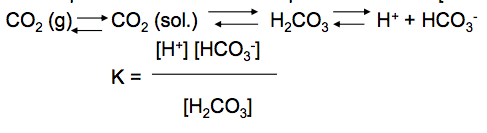
\includegraphics[width=0.8\textwidth]{fig62}
\label{fig62}
\end{figure}

Una part del \ch{CO2} gas�s es dissol en els l�quid corporals (\ch{CO2}
sol). Una part d'aquest \ch{CO2} dissolt en els l�quids corporals
interacciona amb l'aigua donant lloc a �cid carb�nic, que finalment
genera protons i bicarbonat.

L'�cid carb�nic es pot expressar com la fracci� de \ch{CO2} que es troba
dissolta i que interacciona amb l'aigua, obtenint la seg�ent equaci�
(equaci� de Henderson- Hasselbach).

\begin{figure}[H]
\centering
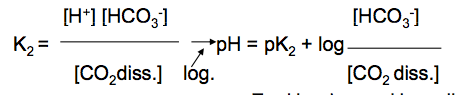
\includegraphics[width=0.6\textwidth]{fig63}
\label{fig63}
\end{figure}

A 38�C la pK d'aquest amortidor �s de 6.1 i tenint en compte que el pH
�s de 7.4 nom�s hem de substituir a l'equaci� de Henderson-Hasselbach.

El quocient de [HCO3-] / [\ch{CO2} dissolt] d�na un valor de 20.
\begin{figure}[H]
\centering
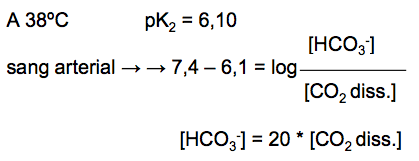
\includegraphics[width=0.6\textwidth]{fig64}
\label{fig64}
\end{figure}

Per una altra banda, la llei de Henry ens diu que:
\begin{figure}[H]
\centering
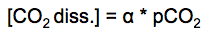
\includegraphics[width=0.4\textwidth]{fig65}
\label{fig65}
\end{figure}

Se sap que a 38�C , $\alpha$ �s $3x10^{-5}$ i que la p\ch{CO2} als
pulmons �s de 40 mmHg, per tant, si substitu�m aquests valors en la
llei de Henry obtenim que:
\begin{center}
  [\ch{CO2} dissolt] = 1.2 mM // [\ch{HCO_3^-}] = 24 mM.
\end{center}

Doncs b�, si el quocient de [\ch{HCO_3^-}]/[\ch{CO2} dissolt] no d�na
un valor de 20,vol dir que hi ha alguna alteraci� en el pH.

\begin{itemize}
\item Si el quocient �s superior a 20, el pH ser� superior a 7.4 i
  tindrem alcalosi (exc�s de bases). L'alcalosi pot ser deguda a un
  exc�s de [\ch{HCO_3^-}] o a un d�ficit de [\ch{CO2} dissolt].

\item Si el quocient �s inferior a 20, el pH ser� inferior a 7.4 i
  tindrem acidosi (exc�s d'�cids). L'acidosi pot ser deguda a un exc�s
  de [\ch{CO2} dissolt] o a un d�ficit de [\ch{HCO_3^-}].
\end{itemize}

Hi ha el�ctrodes selectius que permeten determinar les concentracions
de \ch{H+}, \ch{CO2} i \ch{HCO_3^-}. Coneixent dos dels seg�ents
valors (pH, \ch{HCO_3^-}, \ch{CO2} dissolt, p \ch{CO2}), es poden
calcular els altres. Aqu� trobem dues representacions gr�fiques en qu�
partint de dos d'aquests par�metres, s'ha pogut obtenir un tercer.

La mostra de sang s'obt� de forma anaer�bica amb xeringa de
vidre. Als pulmons hi ha una pressi� de 40 mmHg i a l'aire, la
pressi� no arriba a 1. Per tant, si hi ha un contacte directe entre
aquests dos sistemes amb pressions tan diferents, el \ch{CO2} s'escapa i la
mostra sangu�nia es torna b�sica, ja que el component �cid (\ch{CO2}) ha
marxat. Aix� podria donar lloc a l'obtenci� de falsos positius
d'alcalosi (el resultat indica que hi ha alcalosi, per� realment no
n'hi ha).

Com ja sabem, la sang arterial �s rica en oxigen i la sang venosa �s
rica en \ch{CO2}. Tenint en compte aix�, la sang venosa hauria de ser molt
m�s �cida que l'arterial (si ens fixem en la taula, aix� no �s aix� ja
que els valors s�n molt similars!). La
pres�ncia de tampons fisiol�gics fa que la sang venosa no sigui tan
�cida i que la p\ch{CO2} sigui similar a la que trobem en la sang
arterial. Com a resultat, la sang venosa �s �nicament dues cent�simes
m�s �cida que l'arterial.

La sang arterial es troba molt oxigenada respecte la sang venosa. Aix�
no suposa cap problema ja que l'oxigen no contribueix ni en
l'aportaci� de protons ni en la de grups hidroxils.

\begin{figure}[H]
\centering
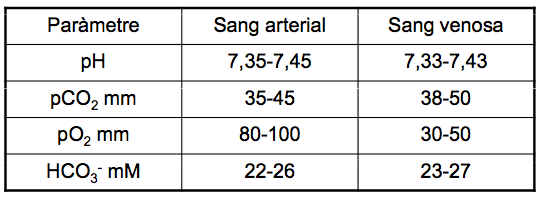
\includegraphics[width=0.8\textwidth]{fig66}
\label{fig66}
\end{figure}

Per controlar la concentraci� de di�xid de carboni utilitzem la
respiraci�:

\begin{itemize}
\item Si ens falta \ch{CO2} --> hipoventilem per tal d'obtenir-ne m�s.
\item Si ens sobra \ch{CO2} --> hiperventilem per tal d'excretar l'exc�s.
\end{itemize}

Per controlar la concentraci� de bicarbonat utilitzem el sistema
urinari.
\begin{itemize}
\item Si ens falta \ch{HCO_3^-} --> reabsorci� als t�buls proximals.
\item Si ens sobra \ch{HCO_3^-} --> orinem.
\end{itemize}

A part de mantenir el pH sanguini, �s essencial controlar tamb� el pH
intracel�lular. Aquest amortidor �cid carb�nic/bicarbonat �nicament t�
utilitat a nivell sanguini, per� no en t� a nivell intracel�lular.

\subsubsection{Amortidor fosfat}
\label{sec:amortidor-fosfat}

La concentraci� de monohidrogenfosfat en plasma �s de 2mM,
aproximadament.
\begin{figure}[H]
\centering
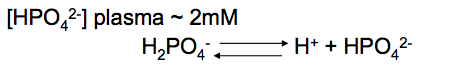
\includegraphics[width=0.75\textwidth]{fig67}
\label{fig67}
\end{figure}

T� tres equilibris possibles: amb un hidrogen (monohidrogenfosfat),
amb dos hidr�gens (dihidrogenfosfat) i amb cap hidrogen.

El pK �s de 6.8, i s'apropa m�s al pH sanguini que l'amortidor �cid
carb�nic/bicarbonat.

En aquest cas, per tal que el pH sanguini sigui de 7.4, s'ha de
mantenir un quocient [\ch{HPO_4^2-}] / [\ch{H2PO_4^-}] de 4. De la mateixa manera
que abans, nom�s cal substituir en l'equaci� de Henderson-Hasselbach.
\begin{figure}[H]
\centering
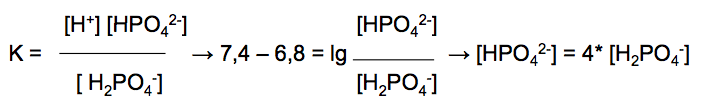
\includegraphics[width=0.75\textwidth]{fig68}
\label{fig68}
\end{figure}

Sabent que la concentraci� de monohidrogenfosfat �s de 2 mM, podem
calcular la de dihidrogenfosfat: 0.5 mM.

�s un tamp� amb menor capacitat tamponadora que l'anterior ja que les
seves esp�cies es troben en concentracions molt baixes. Per� com que
totes les mol�cules que contenen grups fosfats i que es troben dins de
la c�l�lula intervenen en l'equilibri, a nivell intracel�lular �s el
millor tamp�. No ho �s a nivell sanguini!

Algunes d'aquestes mol�cules amb grups fosfat localitzades
intracel�lularment i que intervenen en l'equilibri s�n: �sters triosa
i hexosa, glicerofosfats, fosfol�pids i fosfoprote�nes.

\subsubsection{Prote�nes intracel�lulars}
\label{sec:prot-intr}

Les prote�nes tenen grups ionitzables que es poden protonar i
desprotonar i, per tant, intervenen en el control del pH. Presenten
una gran import�ncia com a tampons intracel�lulars.

\subsubsection{Hemoglobina}
\label{sec:hemoglobina}

�s tracta d'un tamp� plasm�tic. La desoxigenaci� de l'hemoglobina als
teixits incrementa l'afinitat de certs grups d'aquesta mol�cula pels
hidr�gens (\ch{H+}). L'hemoglobina pot controlar els \ch{H+} generats a
l'eritr�cit a trav�s de dos mecanismes:
\begin{itemize}
\item Per compensaci� de c�rrega. L'hemoglobina t� �cids carbox�lics
  que poden agafar protons i tamponar-se.

\item Per p�rdua de c�rrega. La histidina no t� c�rrega i quan capta
  un prot� es carrega, es protona, es torna positiva.
\end{itemize}

\subsubsection{Amortidor ossi}
\label{sec:amortidor-ossi}

\begin{itemize}
\item Medi �cid. Els ossos poden captar els protons dissolent els
  carbonats i els fosfats que formen part d'aquestes estructures. Un
  medi �cid provoca una p�rdua de massa �ssia.

\item Medi b�sic. Incrementa la precipitaci� de carbonats i fosfats,
  fent desapar�ixer els protons de la circulaci�.
\end{itemize}

\subsection{Mecanismes de compensaci� del pH}
\label{sec:mecan-de-comp}

L'increment de protons es compensa per mecanismes que produeixen
bases. Per contra, la baixada de protons es compensa per mecanismes
que produeixen �cids.

L'objectiu �s obtenir una relaci� [\ch{HCO_3^-}] / [\ch{H2CO3}] de 20. Per
aconseguir aquest objectiu existeixen tres mecanismes: metab�lics,
respiratoris i renals.

Els mecanismes metab�lics acostumen a apar�ixer a llarg termini, en
situacions cr�niques. Per contra, els mecanismes respiratoris i renals
apareixen de forma r�pida, immediata.

\subsubsection{Mecanismes metab�lics}
\label{sec:mecan-metab}

Consisteixen en l'activaci� de reaccions enzim�tiques que produeixen o
consumeixen protons.

\subsubsection{Mecanismes respiratoris}
\label{sec:mecan-resp}

Si la concentraci� de bicarbonats incrementa, el quocient [\ch{HCO_3^-}] /
[\ch{CO2} dissolt] ser� superior a 20. Conseq�entment, el pH ser� superior
a 7.4 i ens trobarem en una situaci� d'alcalosi (\ch{OH-} elevats). Si
l'increment de \ch{OH-} arriba al l�quid cefaloraquidi, les neurones
inspirat�ries quedaran inhibides provocant hipoventilaci�. Quan
s'hipoventila, s'incrementa la retenci� de \ch{CO2}. Per tant, el
denominador (\ch{CO2} dissolt) augmenta i es restableix el pH.

L'acidosi pot ser produ�da per una disminuci� de la concentraci� de
bicarbonat o per un exc�s de \ch{CO2} dissolt.

Si la concentraci� de bicarbonats disminueix, el quocient [\ch{HCO_3^-}] /
[\ch{CO2} dissolt] ser� inferior a 20.

Conseq�entment, el pH ser� inferior a 7.4 i ens trobarem en una situaci�
d'acidosi (\ch{H+} elevats). Si l'increment de \ch{H+} arriba al l�quid
cefaloraquidi, les neurones inspirat�ries seran estimulades provocant
hiperventilaci�. Quan s'hiperventila, s'incrementa l'eliminaci� de
\ch{CO2}. Per tant, el denominador (\ch{CO2} dissolt) disminueix i es restableix
el pH.

\subsubsection{Mecanismes renals}
\label{sec:mecanismes-renals}
Podem tenir 2 ocasions:
\begin{itemize}
\item \textbf{Acidosi:} ens interessa augmentar l'excreci� de protons en orina
  i disminuir l'excreci� de bicarbonat en aquest sistema.

\item \textbf{Alcalosi:} ens interessa augmentar l'excreci� de bicarbonat en orina i disminuir l'excreci� de protons en aquest sistema.
\end{itemize}

Aquestes dues situacions fan variar el pH de l'orina des de 4.5 fins a
8.2. Davant aquests canvis de pH, el mecanisme final de defensa �s el
rony�.

Els mecanismes de regulaci� de l'excreci� de protons i bicarbonat:
\begin{itemize}
\item \textbf{Intercanvi \ch{Na+}/\ch{H+}.} La bomba de \ch{Na+}/\ch{K+}/\ch{H+} es localitza als tubs distal i col�lector i es troba controlada per l'aldosterona. Aquesta
  hormona �s alliberada quan falta\ch{Na+}. Quan es necessita \ch{Na+}
  captem \ch{Na+}i, a canvi, s'allibera \ch{K+}/ o \ch{H+}.

Si hi ha acidosi, s'excreten els protons (i no els potassis!). Si hi
ha alcalosi, s'alliberen els potassis (i no protons!). Si hi ha
hiperpotass�mia, els potassis competeixen amb els protons i aix�
dificulta la recuperaci� de l'acidosi, ja que s'excreten potassis i no
protons (o s'excreten protons per� no els suficient com per restablir
el pH).

\item \textbf{Excreci� renal d'amoni (\ch{NH_4^+})}. L'excreci� renal t� lloc al tub
  distal. Les c�l�lules del tub distal s'encarreguen de degradar la
  glutamina (Glu) generant amoni. L'amoni no pot ser excretat de la
  c�l�lula tubular si no �s a trav�s d'un transportador. Per poder
  sortir de les c�l�lules tubulars, l'\ch{NH_4^+} es descompon en amon�ac
  (\ch{NH3}) i protons. L'amon�ac S� �s capa� de creuar la membrana
  d'aquestes c�l�lules. En orina, l'amon�ac r�pidament reacciona amb
  protons generant amoni --> producte que �s detectat en orina.

\item \textbf{Reabsorci� de bicarbonat (\ch{HCO_3^-})}. Si els protons de l'orina,
  procedents de la bomba de \ch{Na+}/\ch{K+}/\ch{H+}, troben bicarbonat, formen �cid
  carb�nic que acabar� generant \ch{CO2} i aigua. El \ch{CO2} produ�t ser�
  absorbit per les c�l�lules tubulars i a trav�s de l'anhidrasa
  carb�nica donar� lloc a �cid carb�nic que es descompon en protons i
  bicarbonat.
\end{itemize}

\subsection{Alteracions de l'equilibri �cid-base}
\label{sec:alter-de-lequ}

Tipus d'afeccions cl�niques:
\begin{itemize}
\item Trastorns que afecten a la concentraci� de bicarbonat:
  patologies \textbf{METAB�LIQUES}.

\item Trastorns que afecten a la concentraci� de di�xid de carboni:
  patologies \textbf{RESPIRAT�RIES}. Si l'afectaci� t� lloc
  directament sobre els protons tamb� rep aquest nom.
\end{itemize}

Segons el resultat de l'equilibri:
\begin{itemize}
\item \textbf{ACIDOSI:} trastorn per un increment dels �cids o per una
  disminuci� de les bases. El pH �s inferior a 7.35.

\item \textbf{ALCALOSI:} trastorn per una disminuci� dels �cids o per un increment
de les bases. El pH �s superior a 7.45.
\end{itemize}

A continuaci� parlarem del concepte de GAP o d�ficit d'anions. El GAP
es calcula a partir de par�metres analitzats en una mostra de sang.

Els ions m�s comuns en sang s�n el SODI, el POTASSI, el CLORUR i el
BICARBONAT. Els dos primers s�n cations i els dos �ltims s�n anions.

 En una situaci� normal, la difer�ncia entre cations i anions hauria
 de ser zero, per� la realitat no �s aquesta. A part dels dos
 anions que hem comentat (clorur i bicarbonat), hi ha d'altres que no
 es consideren per� que tamb� es troben presents:
 \begin{itemize}
 \item Fosfats i sulfats procedents del metabolisme tissular.
 \item Lactat i ceto�cids procedents de l'oxidaci� incomplerta de
   carboni i �cids grassos, respectivament.
 \item Prote�nes, generalment carregades negativament. Implicaci�
   important de l'alb�mina.
 \end{itemize}

El GAP resultant �s precisament per no haver considerat tots aquests
anions/mol�cules carregades negativament!

En una situaci� patol�gica o d'estr�s, aquesta difer�ncia encara es
troba m�s allunyada de zero. Per exemple, quan fem una activitat
f�sica anaer�bica, la producci� de lactat incrementa. Si el lactat no
es considera, el GAP encara ser� m�s gran, ja que en aquesta situaci�
la producci� de lactat �s molt considerable!

\subsubsection{Acidosi metab�lica}
\label{sec:acidosi-metabolica}

En aquest cas tenim el pH per sota de 7.35 i no hi ha exc�s de \ch{CO2},
sin� que tenim una alteraci� amb la concentraci� de bicarbonat.


\begin{itemize}
\item \textbf{Amb GAP normal:} Si el GAP �s normal, l'acidosi
  metab�lica pot ser deguda a diferents motius:
  \begin{enumerate}
  \item P�rdua de bicarbonat (\ch{HCO_3^-}).
La p�rdua de bicarbonat pot tenir lloc a nivell renal o a nivell digestiu.
A nivell renal: el t�bul proximal es troba danyat de manera que el
\ch{HCO_3^-} no s'absorbeix suficientment. El dany al t�bul proximal por ser
degut a una acidosi tubular proximal a�llada o associada al s�ndrome
de Fanconi, a una acidosi per diluci� (en qu� hi ha un increment del
volum plasm�tic), a inhibidors de l'anhidrasa carb�nica o a un
hiperparatiro�disme.

A nivell digestiu: incrementen les secrecions de \ch{HCO_3^-} en el p�ncrees
i en budell prim, generalment per diarrea o per un drenatge del budell
prim.

\item Insuficient regeneraci� de \ch{HCO_3^-} pel t�bul distal.
Aix� pot ser degut a una acidosi tubular distal (les c�l�lules del tub
distal que envolten el nefr� s'acidifiquen sent incapaces d'excretar
protons; �nicament poden llen�ar potassis), a un hipoaldosteronisme o
a l'administraci� de di�r�tics (com l'espironolactona).

\item Subst�ncies productores de \ch{H+} a la dieta. Hi ha sals
  acidificants que formen HCl en el catabolisme, creant un ambient
  �cid. Algunes d'aquestes sals s�n la lisina (Lys), l'arginina (Arg)
  i la histidina (His).
  \end{enumerate}
\item \textbf{Amb GAP elevat:}
  \begin{enumerate}
  \item Excreci� redu�da d'�cids inorg�nics, com a conseq��ncia d'una
    insufici�ncia renal.

  \item Gran producci� d'�cids org�nics. L'excessiva producci� d'�cids
    org�nics pot ser deguda a una acidosi l�ctica o a una cetoacidosi.

Acidosi l�ctica. Es pot produir per una hip�xia tissular deguda a un
xoc, a una an�mia greu, a una intoxicaci� amb CO o a un increment de
l'exercici f�sic. Tamb� pot ser produ�da per ingesta d'etanol, per una
leuc�mia o per un d�ficit cong�nit d'enzims implicats en el
metabolisme.

Cetoacidosi. Deguda a alcoholisme, diabetis o a una situaci� de dejuni.

\item Ingesta de certs productes, com ara etilenglicol, metanol o
  salicilats. Existeixen una s�rie de mecanismes compensatoris per
  disminuir l'acidosi metab�lica. Podem trobar mecanismes
  compensatoris respiratoris o mecanismes compensatoris
  renals. Respecte els mecanismes compensatoris
  respiratoris. Hiperventilaci� per tal d'eliminar el \ch{CO2}. Aix� fa
  incrementar la concentraci� de bicarbonat i, per tant, el pH.

Respecte els mecanismes compensatoris renals. Incrementa l'eliminaci�
d'�cids a trav�s de la bomba de \ch{Na+}/\ch{H+}/\ch{K+}. Tamb� incrementa la
formaci� d'amoni (NH4+) en orina i, per tant, augmenta l'eliminaci� de
protons en forma d'amon�ac (NH3). Per �ltim, hi ha una major
reabsorci� de bicarbonat. Destacar que l'eliminaci� d'�cids a trav�s
de la bomba de Na+/\ch{H+}/\ch{K+} pot ser dificultada per una hiperpotass�mia,
ja que el potassi, que es troba en exc�s �s excretat i els \ch{H+}
s'acumulen, ja que no poden sortir (hi ha una competici� entre els \ch{K+}
i els \ch{H+}).
  \end{enumerate}
\end{itemize}

\subsubsection{Alcalosi metab�lica}
\label{sec:alcalosi-metabolica}

En aquest cas tenim el pH per sobre de 7.45 i hi ha una alteraci� amb
la concentraci� de bicarbonat. Aquesta patologia pot ser deguda als
seg�ents motius:
\begin{enumerate}[\bf 1)]
\item \textbf{Administraci� excessiva de bases}, com per exemple carbonat
  s�dic, citrat en transfusions i anti�cids g�strics.

\item \textbf{Contracci� del volum plasm�tic amb p�rdua gastrointestinal de
  \ch{H+}.} Dues situacions que comporten la contracci� del volum plasm�tic
  i la p�rdua gastrointestinal de protons:
  \begin{itemize}
  \item La p�rdua d'�cid g�stric per la pres�ncia de v�mits
continuats (p�rdua d'HCl). �s a dir, v�mits --> p�rdua de HCl.

\item Una alcalosi cong�nita amb diarrea, tamb� anomenada
clororrea. �s tracta d'un problema hereditari. Els transportadors de
clorur del budell no funcionen, de manera que aquest i� no es pot
captar. Com que el clorur no es pot captar, �s excretat en forma de
diarrea. Com a conseq��ncia, els nivells de clorur al budell
disminueixen. Per poder mantenir la neutralitat, cal aturar els
transportadors de bicarbonat: s'intenta no excretar bicarbonat per tal
de compensar les c�rregues negatives dels clorurs que no es poden
captar. Aix� genera alcalosi.
  \end{itemize}

\item \textbf{Contracci� del volum plasm�tic amb p�rdua renal de \ch{H+}.} Tres
  situacions que comporten la contracci� del volum plasm�tic i la
  p�rdua renal de protons:
  \begin{itemize}
  \item Un tractament prolongat amb di�r�tics.
  \item Una situaci� de posthiperc�pnia. Pr�viament a la
    posthiperc�pnia, ens trobem en situaci� de hiperc�pnia que
    implica: augment de \ch{CO2} que genera acidosi. Es posen en marxa
    mecanismes per captar bases. Si la hiperc�pnia s'atura de cop, en
    la posthiperc�pnia por haver una captaci� excessiva de bases. Aix�
    succeeix en casos de xocs o ofegaments.

  \item Un cas d'hipopotass�mia greu. Quan es necessiti \ch{Na+}, la bomba
    de \ch{Na+}/\ch{H+}/\ch{K+} llan�ar� protons, ja que els potassis es troben
    disminu�ts.
  \end{itemize}
\item \textbf{Hiperfunci� suprarenal.} L'administraci� ex�gena de
  mineralocorticoids i l'hiperaldosteronisme poden conduir a aquesta
  hiperfunci� suprarenal, al igual que els dos s�ndromes comentats a
  continuaci�:
  \begin{itemize}
  \item S�ndrome de Cushing. Patologia relacionada amb el cortisol.
  \item S�ndrome de Bartter. Problema cong�nit que afecta als
    transportadors de \ch{Na+} de la nansa ascendent de Henle. En aquest
    s�ndrome el que succeeix �s que s'activa la bomba de \ch{Na+}/\ch{K+}/\ch{H+} al
    t�bul distal, que per poder captar sodi, llen�a protons i potassi,
    donant lloc a una alcalosi.
  \end{itemize}

\item \textbf{Altres.} Transfusions sangu�nies consecutives.
\end{enumerate}

Existeixen una s�rie de mecanismes compensatoris. Podem trobar mecanismes
compensatoris respiratoris o mecanismes compensatoris renals.
Respecte els mecanismes compensatoris respiratoris. L'augment del pH
provoca la inhibici� del centre respiratori. Aix� fa que
hipoventilem. D'aquesta manera augmenta la retenci� del \ch{CO2}, fent
disminuir el numerador. Aquest mecanisme compensatori t� una
limitaci�: si la pressi� parcial de di�xid de carboni no supera els
55-60 mmHg, es pot produir una caiguda importat de la pressi� parcial
de l'oxigen arterial.

Respecte els mecanismes compensatoris renals. Si hi ha alcalosi, no
s'eliminen �cids per la bomba de \ch{Na+}/\ch{K+}/\ch{H+} sempre i quan hi hagi \ch{K+}
disponible, de manera que tamb� hi ha una limitaci�. Tamb� es pot
disminuir la reabsorci� de bicarbonat i la formaci� de NH4+.

En cas d'alcalosi metab�lica, �s necess�ria l'administraci� de \ch{K+}. En
cas contrari, pot passar el seg�ent:
\begin{itemize}
\item Quan hi ha alcalosi prolongada, si no hi ha suplements orals de
  potassi, la hipopotass�mia causa un alliberament de protons en
  orina. Com a resultat, l'orina apareix �cida --> acid�ria paradoxal
  (l'orina apareix �cida, per� realment ens trobem en una situaci�
  d'alcalosi!).
\end{itemize}

\subsubsection{Acidosi respirat�ria}
\label{sec:acidosi-respiratoria}

Hi ha una interfer�ncia en la capacitat pulmonar per eliminar el \ch{CO2}
que fa incrementar la pressi� parcial del di�xid de carboni
(hiperc�pnia) produint, finalment, acidosi respirat�ria.

\begin{enumerate}[\bf 1)]
\item \textbf{Factors que inhibeixen el centre respiratori.}
  \begin{itemize}
  \item F�rmacs (narc�tics, barbit�rics).
  \item Infeccions (encefalitis, meningitis).
  \item Traumatismes, tumors i degeneraci� del SNC.
  \item Estats de coma.
  \end{itemize}
\item \textbf{Factors que afecten els pulmons.}
  \begin{itemize}
  \item Obstrucci� pulmonar cr�nica.
  \item Fibrosi pulmonar.
  \item Estats asm�tics.
  \item Infeccions pulmonars greus.
  \item Pneumot�rax i vessament pleural.
  \end{itemize}
\item \textbf{Altres}
  \begin{itemize}
  \item Laringospasmes.
  \item Tumors en vies respirat�ries superiors.
  \item Greus distensions abdominals.
  \item Obesitat extrema.
  \item Trastorn del somni (apnea nocturna)
  \end{itemize}
\end{enumerate}

Existeixen una s�rie de mecanismes compensatoris. Podem trobar
mecanismes compensatoris respiratoris o mecanismes compensatoris
renals. S�n iguals que els utilitzats durant l'acidosi metab�lica.

Respecte els mecanismes compensatoris respiratoris. S�n poc
eficients. Rarament funcionen perqu� els problemes s�n respiratoris.

Respecte els mecanismes compensatoris renals. Augmenta l'eliminaci�
d'�cids amb l'antiport \ch{Na+}/\ch{H+}. Augmenta l'eliminaci� en forma
d'amoni. Incrementa la reabsorci� de \ch{HCO_3^-}.

\subsubsection{Alcalosi respirat�ria}
\label{sec:alcal-resp}

Aquesta patologia �s provocada per una hiperventilaci�, que fa
incrementar la freq��ncia, la qual cosa comporta la p�rdua o la
baixada de di�xid de carboni. L'eliminaci� incrementada de di�xid de
carboni provoca hipoc�pnia, per la disminuci� de la pressi� parcial
del di�xid de carboni. A m�s, si el denominador disminueix, el
numerador (concentraci� de bicarbonat) incrementa. Aix� fa incrementar
el pH.

\begin{enumerate}[\bf 1)]
\item \textbf{Factors que estimulen el centre respiratori.}
  \begin{itemize}
  \item Ansietat/Hist�ria.
  \item Accidents vasculars cerebrals (insufici�ncia).
  \item Septic�mia per bacteris gram negatius.
  \item Encefalopatia metab�lica.
  \item Infeccions del SNC.
  \item Hip�xia greu (per asma, pneum�nia, grans al�ades).
  \item Hipotensi�.
  \item Compressi� respirat�ria a una acidosi metab�lica.
  \item Progesterona alliberada durant l'embar�s.
  \end{itemize}
\item \textbf{Administraci� de f�rmacs.}
  \begin{itemize}
  \item Catecolamines: ansietat, estr�s.
  \item F�rmacs: salicilats, aminofil�lina.
  \item Nicotina.
  \end{itemize}

\item \textbf{Ventilaci� mec�nica excessiva.}
\end{enumerate}

Es compensa amb tampons tissulars o renals que disminueixen l'eliminaci� d'�cids
amb l'antiport \ch{Na+}/\ch{H+}, disminueix la formaci� de NH4+ i disminueix la
reabsorci� \ch{HCO_3^-}.

Per �ltim comentar que en casos d'acidosi, els clorurs en orina es
troben incrementats. En casos d'acidosi, el pH de l'orina baixa per
compensaci� renal. Hi ha reabsorci� de bicarbonat, la qual cosa fa que
augmenti la carga negativa: els transportadors de clorur s'aturen ja
que si no tindr�em un exc�s de c�rrega negativa i aquests llavors es
perden per orina.


%===============================================================
%===============================================================
\newpage
\phantomsection
\addcontentsline{toc}{part}{Refer�ncies}
\begin{multicols}{2}
\bibliography{bibbac} 
\bibliographystyle{authordate3}
\end{multicols}

\end{document}

Els de BIOMED fem un parcial. Val un 10\% extra.

El final �s 60 preguntes tipus test, 3 preguntes curtes de cada part +
10 preguntes de pr�ctiques.

Treball: Vicent Casad�